
\section{Results and Discussion}
\subsection{Dataset Analysis}
The data for this work was collected as described in Section \ref{sec:mdethods:data_collection}, resulting in a dataset containing 90 colon biopsy samples, their associated H\&E stained images, their FTIR spectral images with absorption intensities at 801 wavenumbers from $1000$-$1800$ cm$^{-1}$, and their histopathological classification as either normal, hyperplastic, adenomatous or cancerous tissue \cite{nallala_high-resolution_2016}. Notably, this histopathological classification was made according to the most severe tissue condition present within the sample, so a sample containing only 2-3\% cancerous tissue would still be classified as cancerous. We therefore expect many pixels within the spectral images to be incorrectly labelled, which could contribute to the very similar average spectra in all classes as shown in Figure \ref{fig:dataset_differences}.  \\

\noindent
False-colour images for samples were generated by taking the intensities for each pixel at high-variance wavenumbers $1080$cm$^{-1}$, $1230$cm$^{-1}$ and $1600$cm$^{-1}$, and then scaling them to values between $0$ and $1$, centred around $0.5$ according to the standard deviation of intensity values at that wavenumber throughout the sample. For each classification, one of these false-colour images along with its associated H\&E stain is presented in Figure \ref{fig:IR_and_HE_categories}. This figure both demonstrates the boundary of stroma regions and the locations of H\&E image folds preventing perfect alignment. Only the non-stroma regions are used for subsequent prediction analysis.

\begin{figure}[htb]
  \centering
  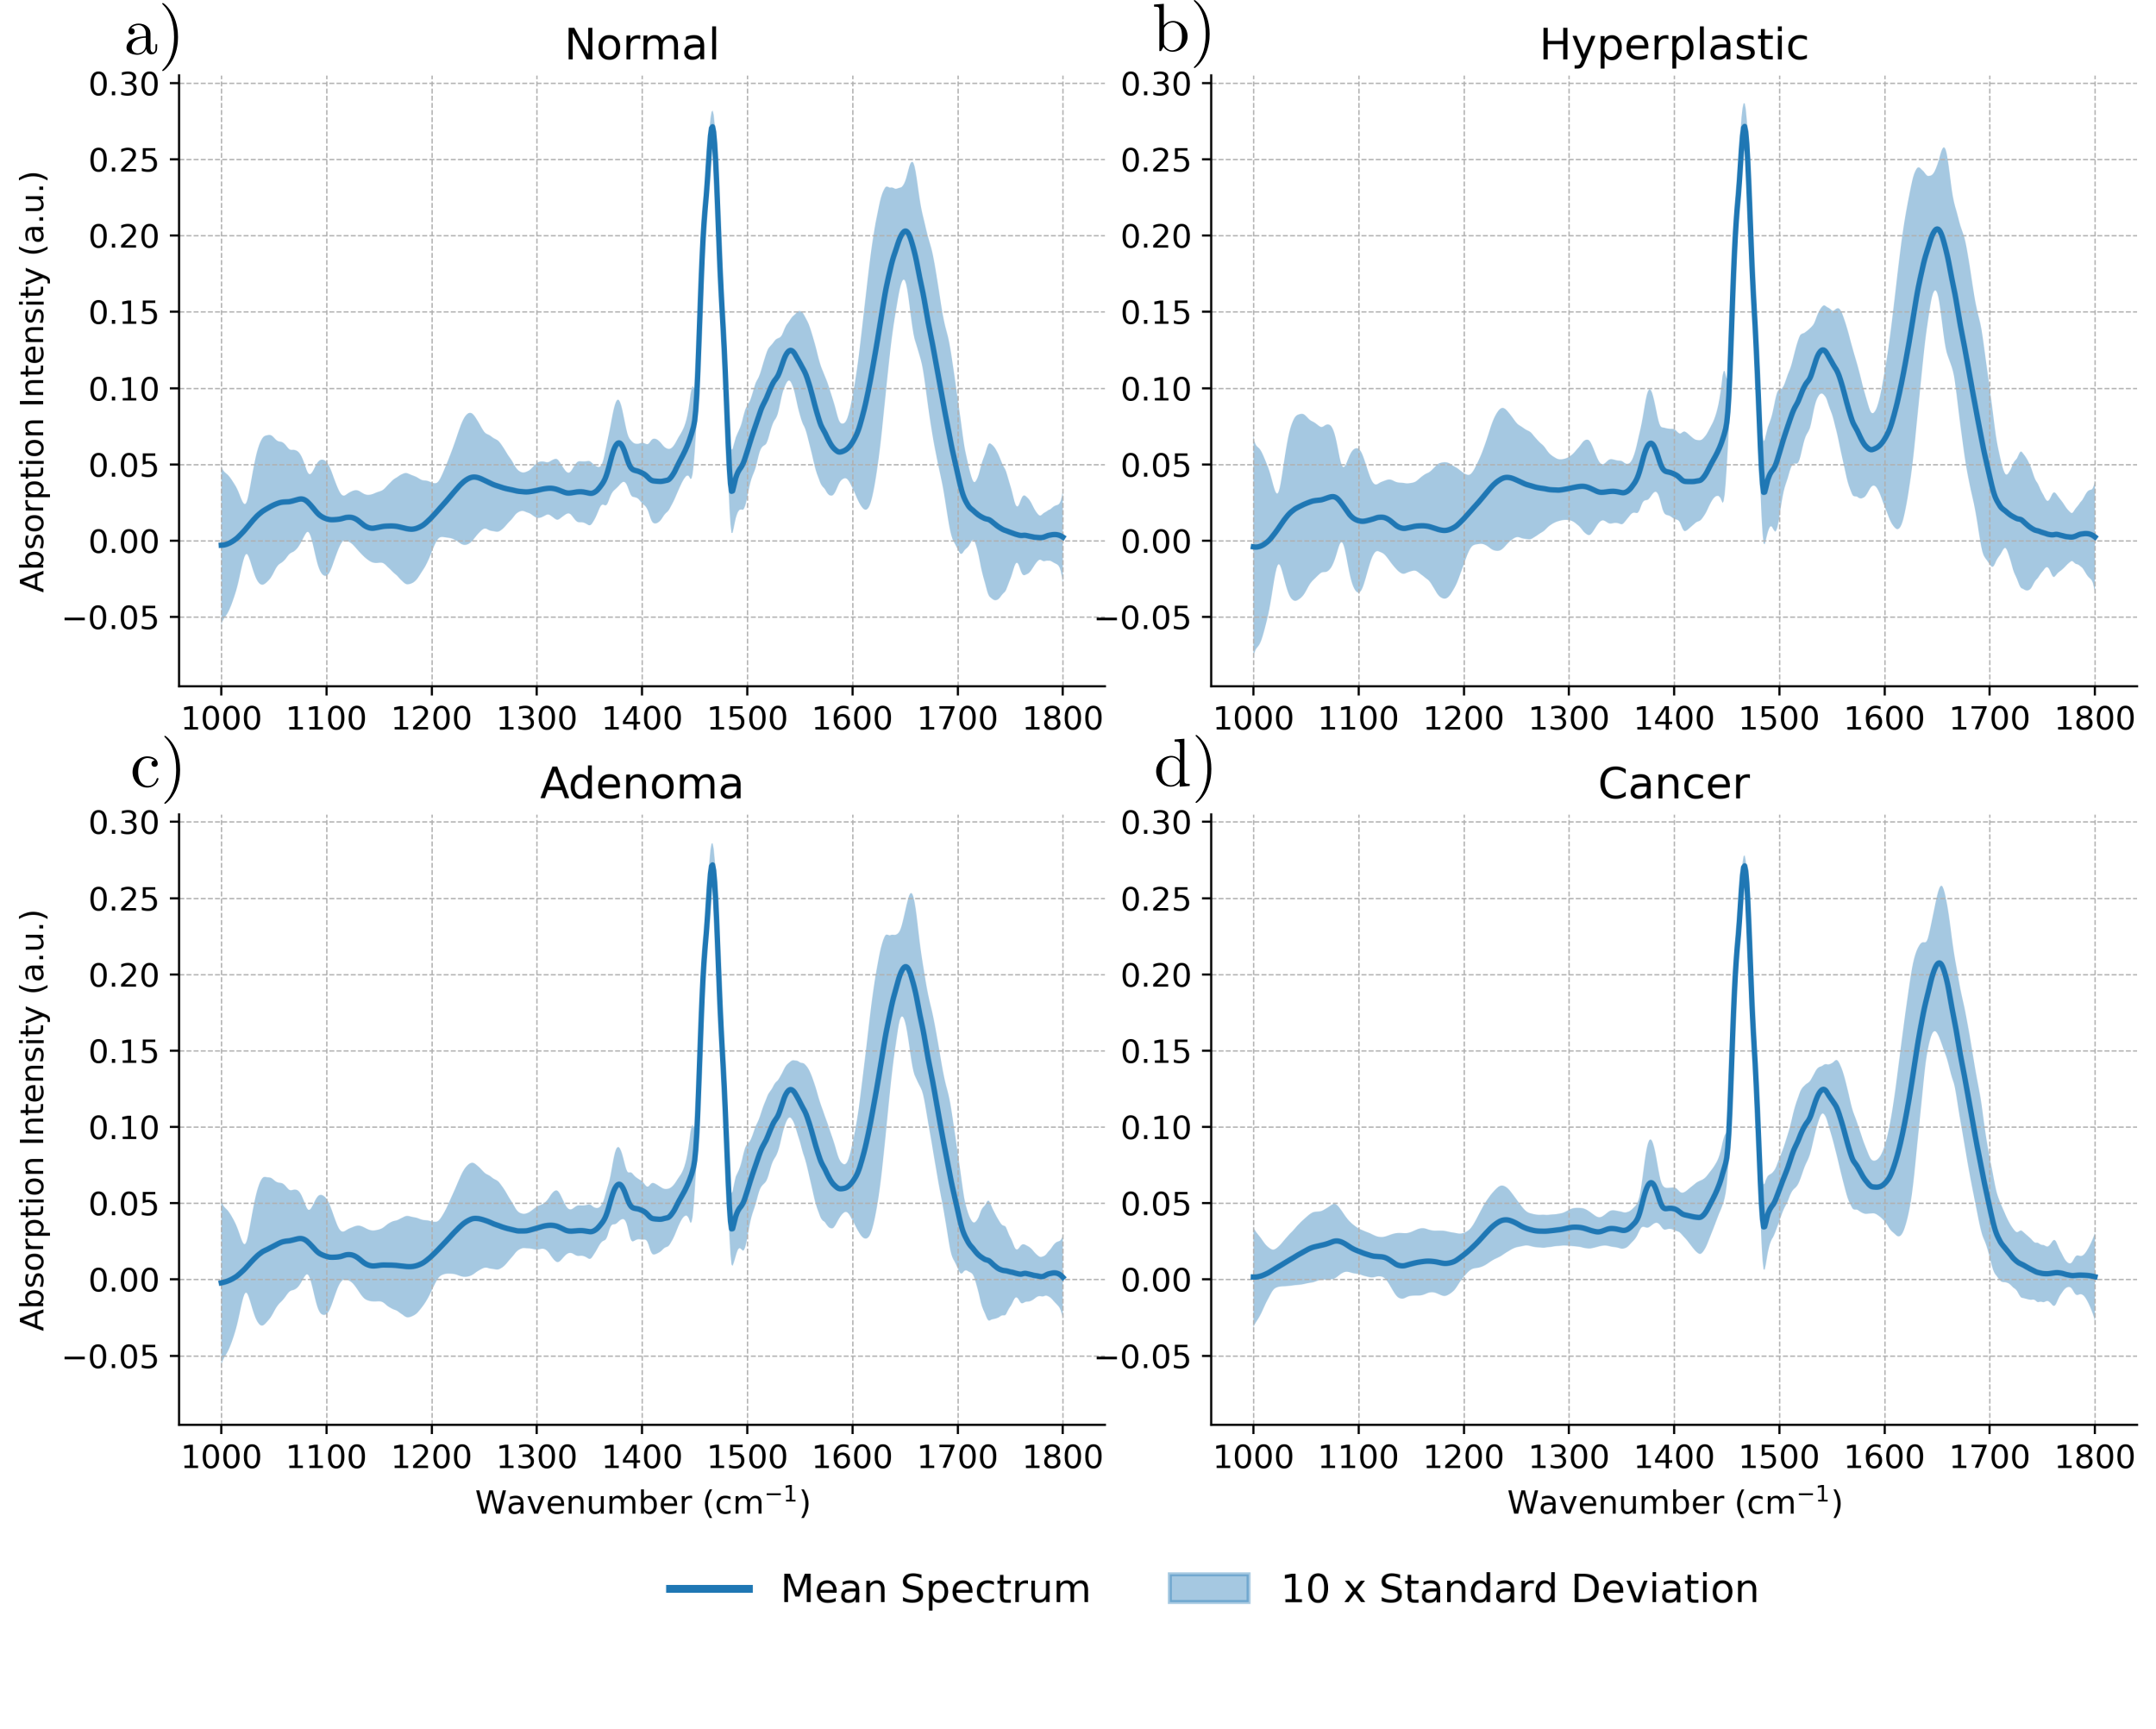
\includegraphics[width=1\textwidth]{Images/Dataset_Class_Differences.png}
  \caption{Plots showing the mean and standard deviation of the FTIR spectral intensities across each class. The cancerous sample spectra are seen to have slightly smaller standard deviations than other classifications. The only visually discernable difference between the mean spectra is around 1120 cm$^{-1}$, where the cancerous spectra does not show a small peak which can be observed in the spectra associated with the other classes.}
  \label{fig:dataset_differences}
\end{figure}

\begin{figure}[htbp] 
    \centering 
    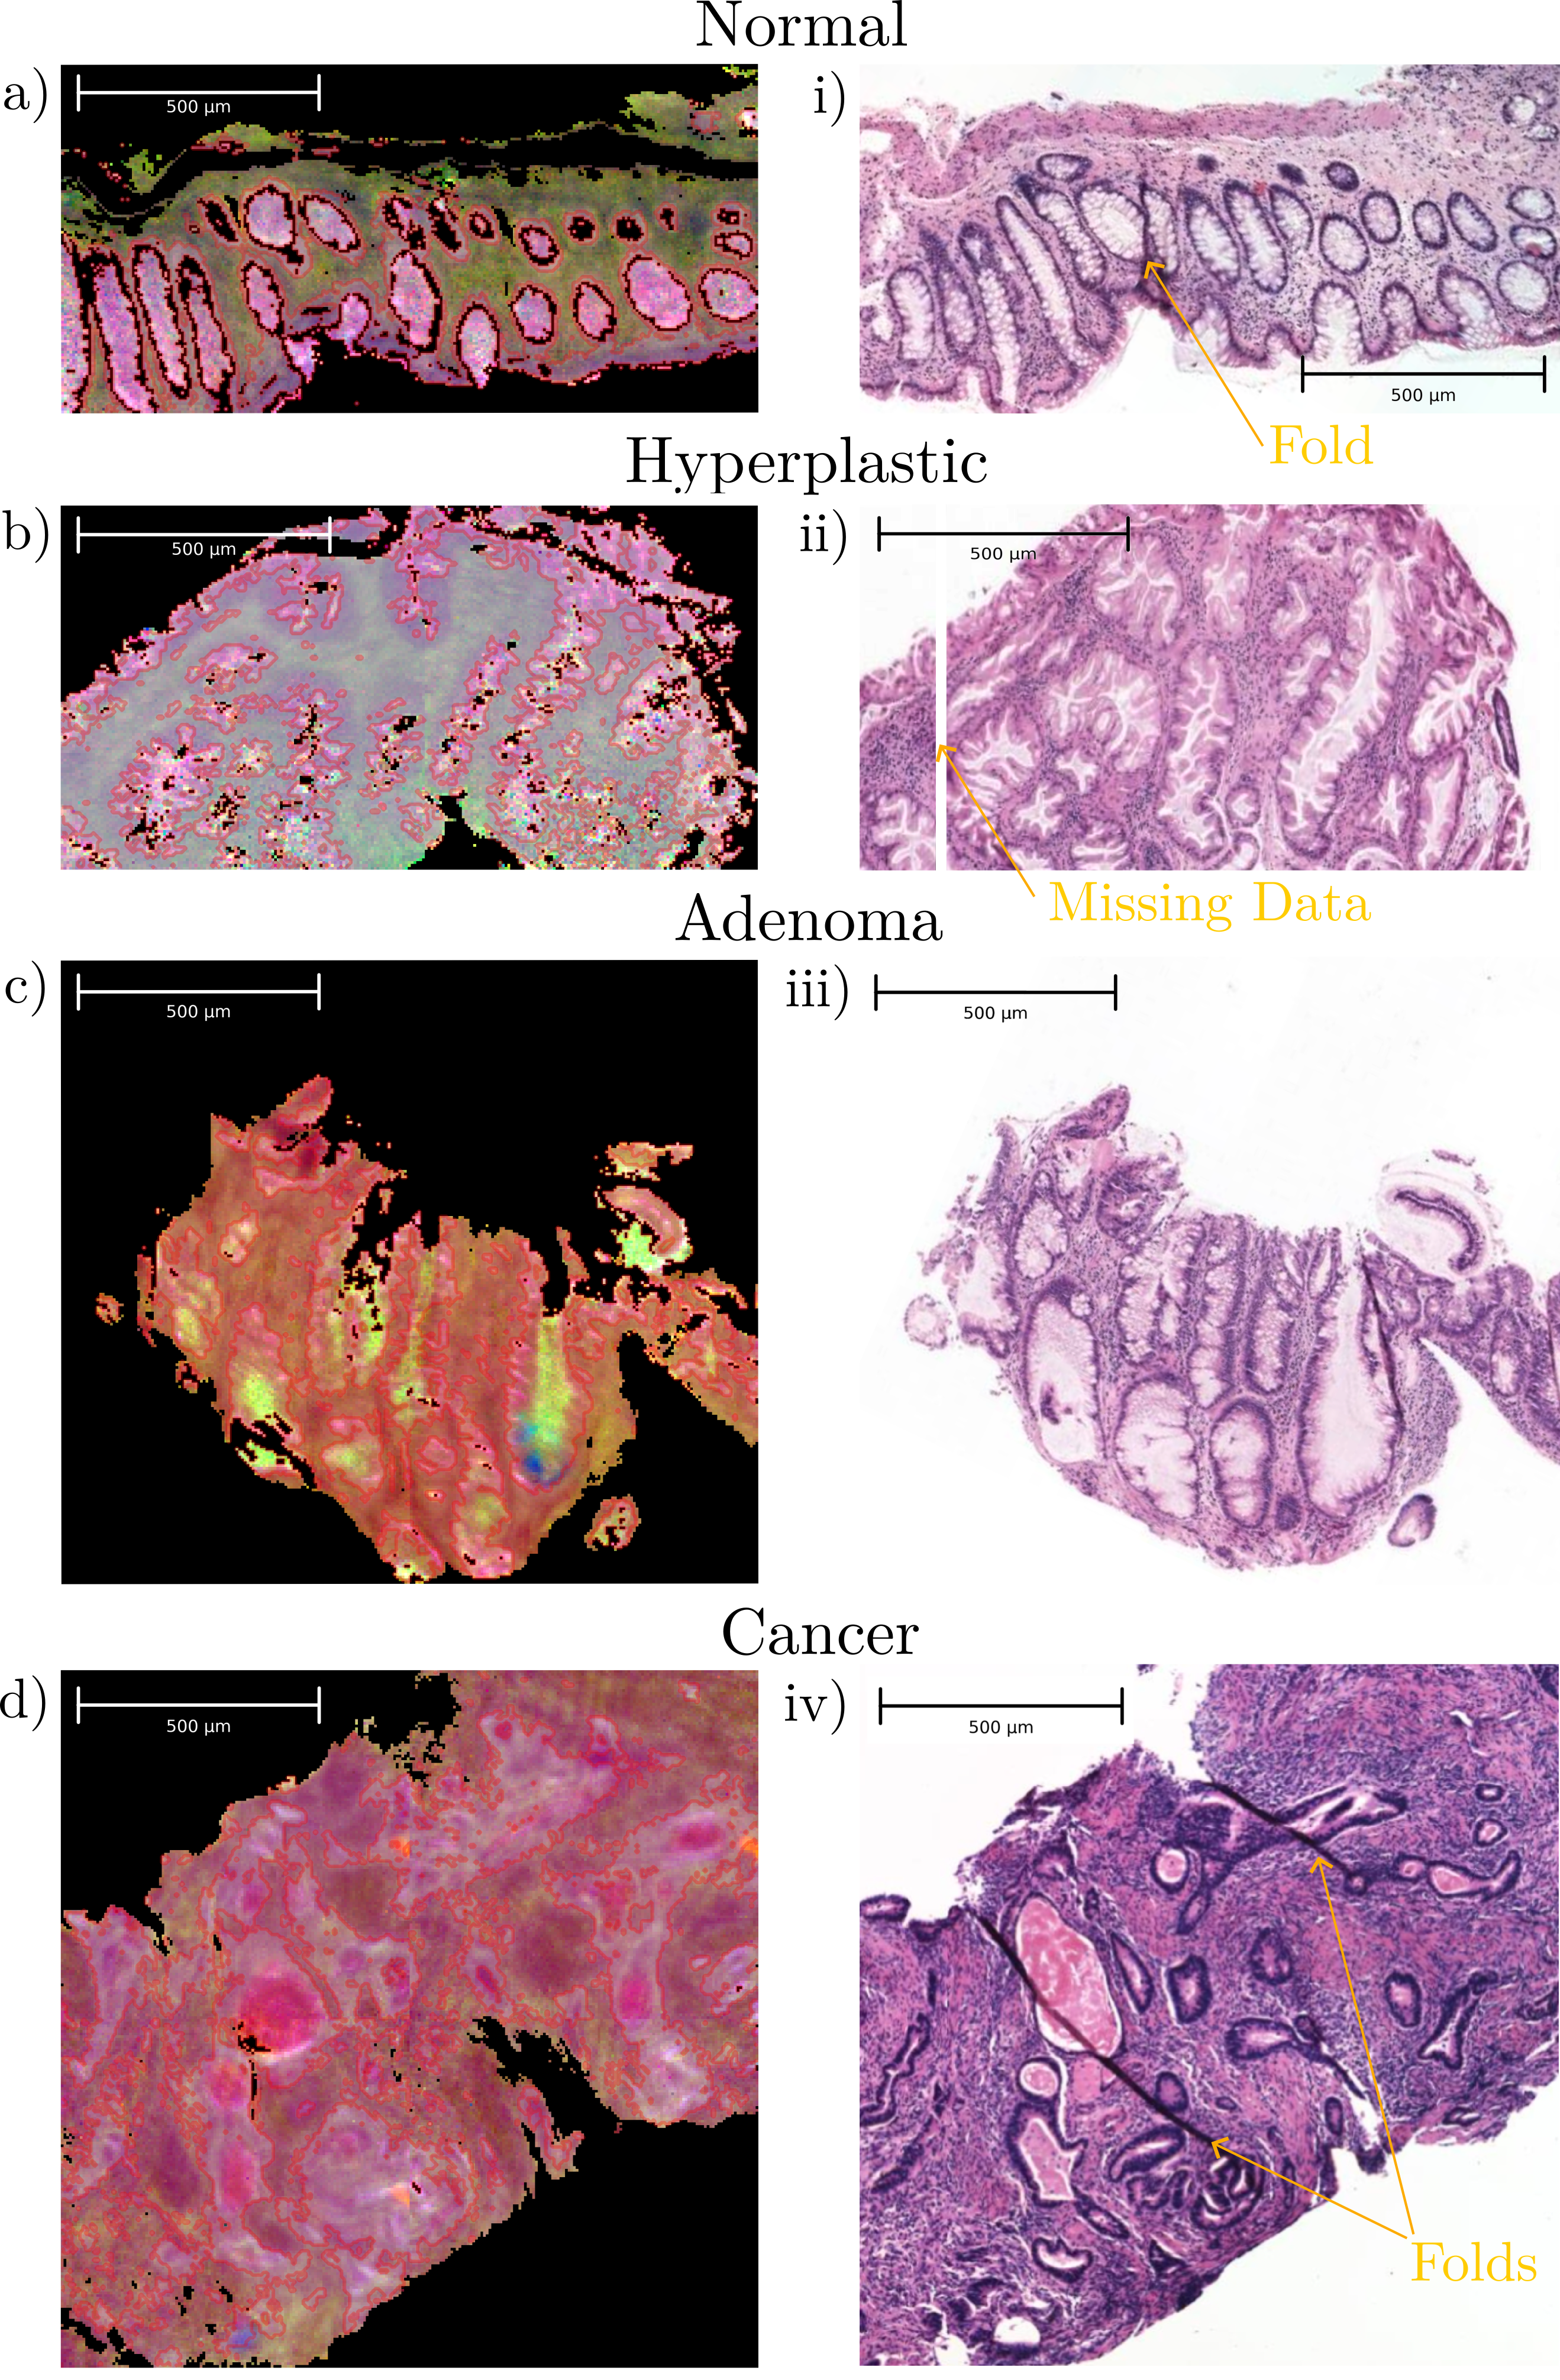
\includegraphics[width=0.85\textwidth]{Images/IR_and_HE_categories.png} 
    \caption{Sections a-d show false-colour FTIR images of colon biopsy samples - one per labelling classification. Each of these has non-stroma regions surrounded by red outlines and highlighted with a white accent. Sections i-iv show the corresponding aligned H\&E images. Note that the H\&E images in sections i and iv show folding defects, and information for a small stripe of the image in section ii is missing, so is blanked.} 
    \label{fig:IR_and_HE_categories} 
\end{figure}


\newpage

\subsection{Classification Methods}
\subsubsection{Traditional Classification Methods}
The classification methods described in §\ref{sec:methods:baseline_classification} and §\ref{sec:methods:trad_ML_usage} were applied to the dataset to produce both four-class and binary classification performance results. In all cases, the default hyperparameter values were used. The performance results from these experiments are presented in Tables \ref{table:quad_results_full} and \ref{table:binary_results_full} respectively. These tables also show the performance of the SCNN method applied in this work for comparison.

% \begin{table}[ht]
% \centering
% \begin{tabular}{lcccc}
% \toprule
% Metric & Normal & Hyperplastic & Adenoma & Cancer \\
% \midrule
% Sensitivity       & $0.238\pm0.032$ & $0.396\pm0.138$ & $0.310\pm0.056$ & $0.829\pm0.114$ \\
% Specificity       & $0.853\pm0.040$ & $0.823\pm0.098$ & $0.812\pm0.088$ & $0.703\pm0.067$ \\
% Accuracy          & $0.733\pm0.030$ & $0.755\pm0.073$ & $0.562\pm0.047$ & $0.722\pm0.068$ \\
% False Positive Rate & $0.147\pm0.040$ & $0.177\pm0.098$ & $0.188\pm0.088$ & $0.297\pm0.067$ \\
% \midrule
% Overall Weighted Accuracy  & \multicolumn{4}{c}{$0.443\pm0.062$} \\
% \bottomrule
% \end{tabular}
% \caption{The four-classification performance (mean $\pm$ std) across folds achieved by both the MSE and cosine similarity spectral matching methods. Note, performances of both methods are identical to 3 s.f. so only one table is shown.}
% \label{table:spectral_mathching_1}
% \end{table}

% \begin{table}[ht]
% \centering
% \begin{tabular}{lcc}
% \toprule
% Metric & Non-Cancer& Cancer \\
% \midrule
% Sensitivity         & $0.703\pm0.067$ & $0.829\pm0.114$ \\
% Specificity         & $0.829\pm0.114$ & $0.703\pm0.067$ \\
% Accuracy            & $0.722\pm0.068$ & $0.722\pm0.068$ \\
% False Positive Rate & $0.171\pm0.114$ & $0.297\pm0.067$ \\
% \midrule
% Overall Weighted Accuracy    & \multicolumn{2}{c}{$0.766\pm0.080$} \\
% \bottomrule
% \end{tabular}
% \caption{The binary classification performance (mean $\pm$ std)
% across folds achieved by both the MSE and cosine similarity spectral matching
% methods. These results follow from mapping four-classification predictions into cancer / non-cancer classifications. Note, the performances of both methods are identical to 3 s.f. so only one table
% is shown.}
% \label{table:spectral_matching_2}
% \end{table}

% \subsection{Traditional Machine Learning Approaches}
% Previous, unpublished work on this dataset by Tiago Azevedo explored the application of traditional machine learning methods to achieve spectral classifications. Azevedo used PCA (§\ref{sec:methods:pca}) to extract 25-dimensional representations of the dataset before applying LDA (§\ref{sec:methods:lda}) and XGBoost (§\ref{sec:methods:xgboost}) to categorise test set samples. Azevedo used 10-fold cross-validation for their testing, so for comparability, their results were reproduced for this work using the 4-fold cross-validation method outlined in §\ref{sec:methods:data_split}, and the results of this analysis are presented in 
% Table \ref{tab:trad_ml_performance}. The original 10-fold performance results can be found in appendix \ref{appendix:Tiago}.



% \begin{table}[ht]
% \centering
% \begin{tabular}{lcccc}
% \toprule
% Metric & Normal & Hyperplastic & Adenoma & Cancer \\
% \midrule
% Sensitivity         & $0.430\pm0.043$ & $0.230\pm0.099$ & $0.800\pm0.075$ & $0.440\pm0.294$ \\
% Specificity         & $0.890\pm0.062$ & $0.950\pm0.041$ & $0.550\pm0.174$ & $0.930\pm0.042$ \\
% Accuracy            & $0.800\pm0.052$ & $0.830\pm0.044$ & $0.670\pm0.090$ & $0.860\pm0.071$ \\
% False Positive Rate & $0.110\pm0.062$ & $0.050\pm0.041$ & $0.450\pm0.174$ & $0.070\pm0.042$ \\
% \midrule
% Overall Weighted Accuracy & \multicolumn{4}{c}{$0.476\pm0.079$} \\
% \bottomrule
% \end{tabular}
% \caption{The four-classification performance (mean $\pm$ std) across folds achieved by PCA $>$ LDA. Only PCA $>$ LDA results are shown.}
% \label{table:pca_lda_4class_performance}
% \end{table}

% \begin{table}[ht]
% \centering
% \begin{tabular}{lcccc}
% \toprule
% Metric & Normal & Hyperplastic & Adenoma & Cancer \\
% \midrule
% Sensitivity         & $0.470\pm0.096$ & $0.350\pm0.090$ & $0.770\pm0.051$ & $0.590\pm0.075$ \\
% Specificity         & $0.880\pm0.030$ & $0.900\pm0.047$ & $0.710\pm0.094$ & $0.940\pm0.054$ \\
% Accuracy            & $0.800\pm0.028$ & $0.810\pm0.034$ & $0.740\pm0.066$ & $0.880\pm0.050$ \\
% False Positive Rate & $0.120\pm0.030$ & $0.100\pm0.047$ & $0.290\pm0.094$ & $0.060\pm0.054$ \\
% \midrule
% Overall Weighted Accuracy & \multicolumn{4}{c}{$0.544\pm0.053$} \\
% \bottomrule
% \end{tabular}
% \caption{The four-classification performance (mean $\pm$ std) across folds achieved by PCA $>$ XGBoost. Only PCA $>$ XGBoost results are shown.}
% \label{table:pca_xgb_4class_performance}
% \end{table}

% \begin{table}[ht]
% \centering
% \begin{tabular}{lcccc}
% \toprule
% Metric & Normal & Hyperplastic & Adenoma & Cancer \\
% \midrule
% Sensitivity         & $0.50\pm0.093$ & $0.38\pm0.115$ & $0.78\pm0.048$ & $0.61\pm0.079$ \\
% Specificity         & $0.89\pm0.025$ & $0.91\pm0.031$ & $0.71\pm0.089$ & $0.94\pm0.048$ \\
% Accuracy            & $0.81\pm0.022$ & $0.83\pm0.009$ & $0.75\pm0.064$ & $0.89\pm0.048$ \\
% False Positive Rate & $0.11\pm0.025$ & $0.09\pm0.031$ & $0.29\pm0.089$ & $0.06\pm0.048$ \\
% \midrule
% Overall Weighted Accuracy & \multicolumn{4}{c}{$0.568\pm0.058$} \\
% \bottomrule
% \end{tabular}
% \caption{The four-classification performance (mean $\pm$ std) across folds achieved by XGBoost. Only XGBoost results are shown.}
% \label{table:xgb_4class_performance}
% \end{table}

% \begin{table}[ht]
% \centering
% \begin{tabular}{llcccc}
% \toprule
% Method & Metric & Normal & Hyperplastic & Adenoma & Cancer \\
% \midrule
% PCA $\to$ LDA & Sensitivity         & $0.430\pm0.043$ & $0.230\pm0.099$ & $0.800\pm0.075$ & $0.440\pm0.294$ \\
%  & Specificity         & $0.890\pm0.062$ & $0.950\pm0.041$ & $0.550\pm0.174$ & $0.930\pm0.042$ \\
%  & Accuracy            & $0.800\pm0.052$ & $0.830\pm0.044$ & $0.670\pm0.090$ & $0.860\pm0.071$ \\
%  & False Positive Rate & $0.110\pm0.062$ & $0.050\pm0.041$ & $0.450\pm0.174$ & $0.070\pm0.042$ \\
%  & Overall Weighted Accuracy & \multicolumn{4}{c}{$0.476\pm0.079$} \\
% \midrule
% PCA $\to$ XGB & Sensitivity         & $0.470\pm0.096$ & $0.350\pm0.090$ & $0.770\pm0.051$ & $0.590\pm0.075$ \\
%  & Specificity         & $0.880\pm0.030$ & $0.900\pm0.047$ & $0.710\pm0.094$ & $0.940\pm0.054$ \\
%  & Accuracy            & $0.800\pm0.028$ & $0.810\pm0.034$ & $0.740\pm0.066$ & $0.880\pm0.050$ \\
%  & False Positive Rate & $0.120\pm0.030$ & $0.100\pm0.047$ & $0.290\pm0.094$ & $0.060\pm0.054$ \\
%  & Overall Weighted Accuracy & \multicolumn{4}{c}{$0.544\pm0.053$} \\
% \midrule
% XGBoost & Sensitivity         & $0.50\pm0.093$ & $0.38\pm0.115$ & $0.78\pm0.048$ & $0.61\pm0.079$ \\
%  & Specificity         & $0.89\pm0.025$ & $0.91\pm0.031$ & $0.71\pm0.089$ & $0.94\pm0.048$ \\
%  & Accuracy            & $0.81\pm0.022$ & $0.83\pm0.009$ & $0.75\pm0.064$ & $0.89\pm0.048$ \\
%  & False Positive Rate & $0.11\pm0.025$ & $0.09\pm0.031$ & $0.29\pm0.089$ & $0.06\pm0.048$ \\
%  & Overall Weighted Accuracy & \multicolumn{4}{c}{$0.568\pm0.058$} \\
% \bottomrule
% \end{tabular}
% \caption{Comparison of four-classification performance (mean $\pm$ std) across folds for PCA $\to$ LDA, PCA $\to$ XGBoost, and XGBoost.}
% \label{table:tab:trad_ml_performance}
% \end{table}

% \begin{table}[ht]
%     \centering
%     \begin{tabular}{llcc}
%         \toprule
%         Method                & Metric               & Non‐Cancer           & Cancer              \\
%         \midrule
%         \multirow{5}{*}{PCA $\rightarrow$ LDA} 
%                               & Sensitivity          & $0.93 \pm 0.042$     & $0.44 \pm 0.294$    \\
%                               & Specificity          & $0.44 \pm 0.294$     & $0.93 \pm 0.042$    \\
%                               & Accuracy             & $0.86 \pm 0.071$     & $0.86 \pm 0.071$    \\
%                               & False Positive Rate  & $0.56 \pm 0.294$     & $0.07 \pm 0.042$    \\
%                               & Overall Accuracy     & \multicolumn{2}{c}{$0.687 \pm 0.162$}           \\
%         \midrule
%         \multirow{5}{*}{PCA $\rightarrow$ XGB} 
%                               & Sensitivity          & $0.93 \pm 0.055$     & $0.60 \pm 0.075$    \\
%                               & Specificity          & $0.60 \pm 0.075$     & $0.93 \pm 0.055$    \\
%                               & Accuracy             & $0.89 \pm 0.049$     & $0.89 \pm 0.049$    \\
%                               & False Positive Rate  & $0.40 \pm 0.075$     & $0.07 \pm 0.055$    \\
%                               & Overall Accuracy     & \multicolumn{2}{c}{$0.769 \pm 0.049$}           \\
%         \midrule
%         \multirow{5}{*}{XGB} 
%                               & Sensitivity          & $0.94 \pm 0.047$     & $0.61 \pm 0.084$    \\
%                               & Specificity          & $0.61 \pm 0.084$     & $0.94 \pm 0.047$    \\
%                               & Accuracy             & $0.89 \pm 0.049$     & $0.89 \pm 0.049$    \\
%                               & False Positive Rate  & $0.39 \pm 0.084$     & $0.06 \pm 0.047$    \\
%                               & Overall Accuracy     & \multicolumn{2}{c}{$0.773 \pm 0.060$}           \\
%         \bottomrule
%     \end{tabular}
%     \caption{Comparison of binary classification performance (mean $\pm$ std) for PCA $\rightarrow$ LDA, PCA $\rightarrow$ XGB, and XGB.}
%     \label{tab:binary_perf}
% \end{table}

% \noindent






\subsection{A Scale-Invariant Convolutional Neural Network Approach}

The SCNN architecture described in §\ref{sec:methods:scnn} was trained on each dataset fold (§\ref{sec:methods:data_split}) using a weighted cross-entropy loss to predict the four-class classification of each spectral pixel. Significant regularisation and hyperparameter tuning were required to achieve reliable model convergence. For this tuning, random search was employed to identify hyperparameter ranges which consistently produced converging models. These ranges are presented in Table \ref{tab:scnn_class_hyper_ranges}. Random search was then again employed within each of these hyperparameter ranges to produce a set of converged models. Figure \ref{fig:val_fold_boxes} shows the OWAs these models achieve on each dataset fold. The difficulty in achieving model convergence is likely due to the incorrect labelling of many pixels in the dataset. It is therefore thought that future work could investigate the use of an ordinal loss function \cite{castagnos_simple_2022,polat_class_2025} to additionally penalise predictions more severe than the true label.

\begin{table}[htbp]
    \centering
    \begin{tabular}{l l l}
    \hline
    Parameter & Distribution & Numeric Bounds \\
    \hline
    Dropout Rate        & Log-uniform         & $0.01 \rightarrow 0.30$   \\
    Adenoma Entropy Weight    & Uniform              & $0.05 \rightarrow 0.40$   \\
    Leak Rate            & Log-uniform         & $1\times 10^{-6} \rightarrow 0.80$ \\
    Learning Rate       & Log-uniform         & $1\times 10^{-6} \rightarrow 0.05$ \\
    Scheduler Step Size & Integer uniform     & $5 \rightarrow 20$        \\
    Weight Decay        & Log-uniform         & $1\times 10^{-5} \rightarrow 0.50$ \\
    \hline
    \end{tabular}
    \caption{Tuned hyperparameter ranges used for SCNN model training.} 
    \label{tab:scnn_class_hyper_ranges}
\end{table}

\begin{figure}[htbp] 
    \centering 
    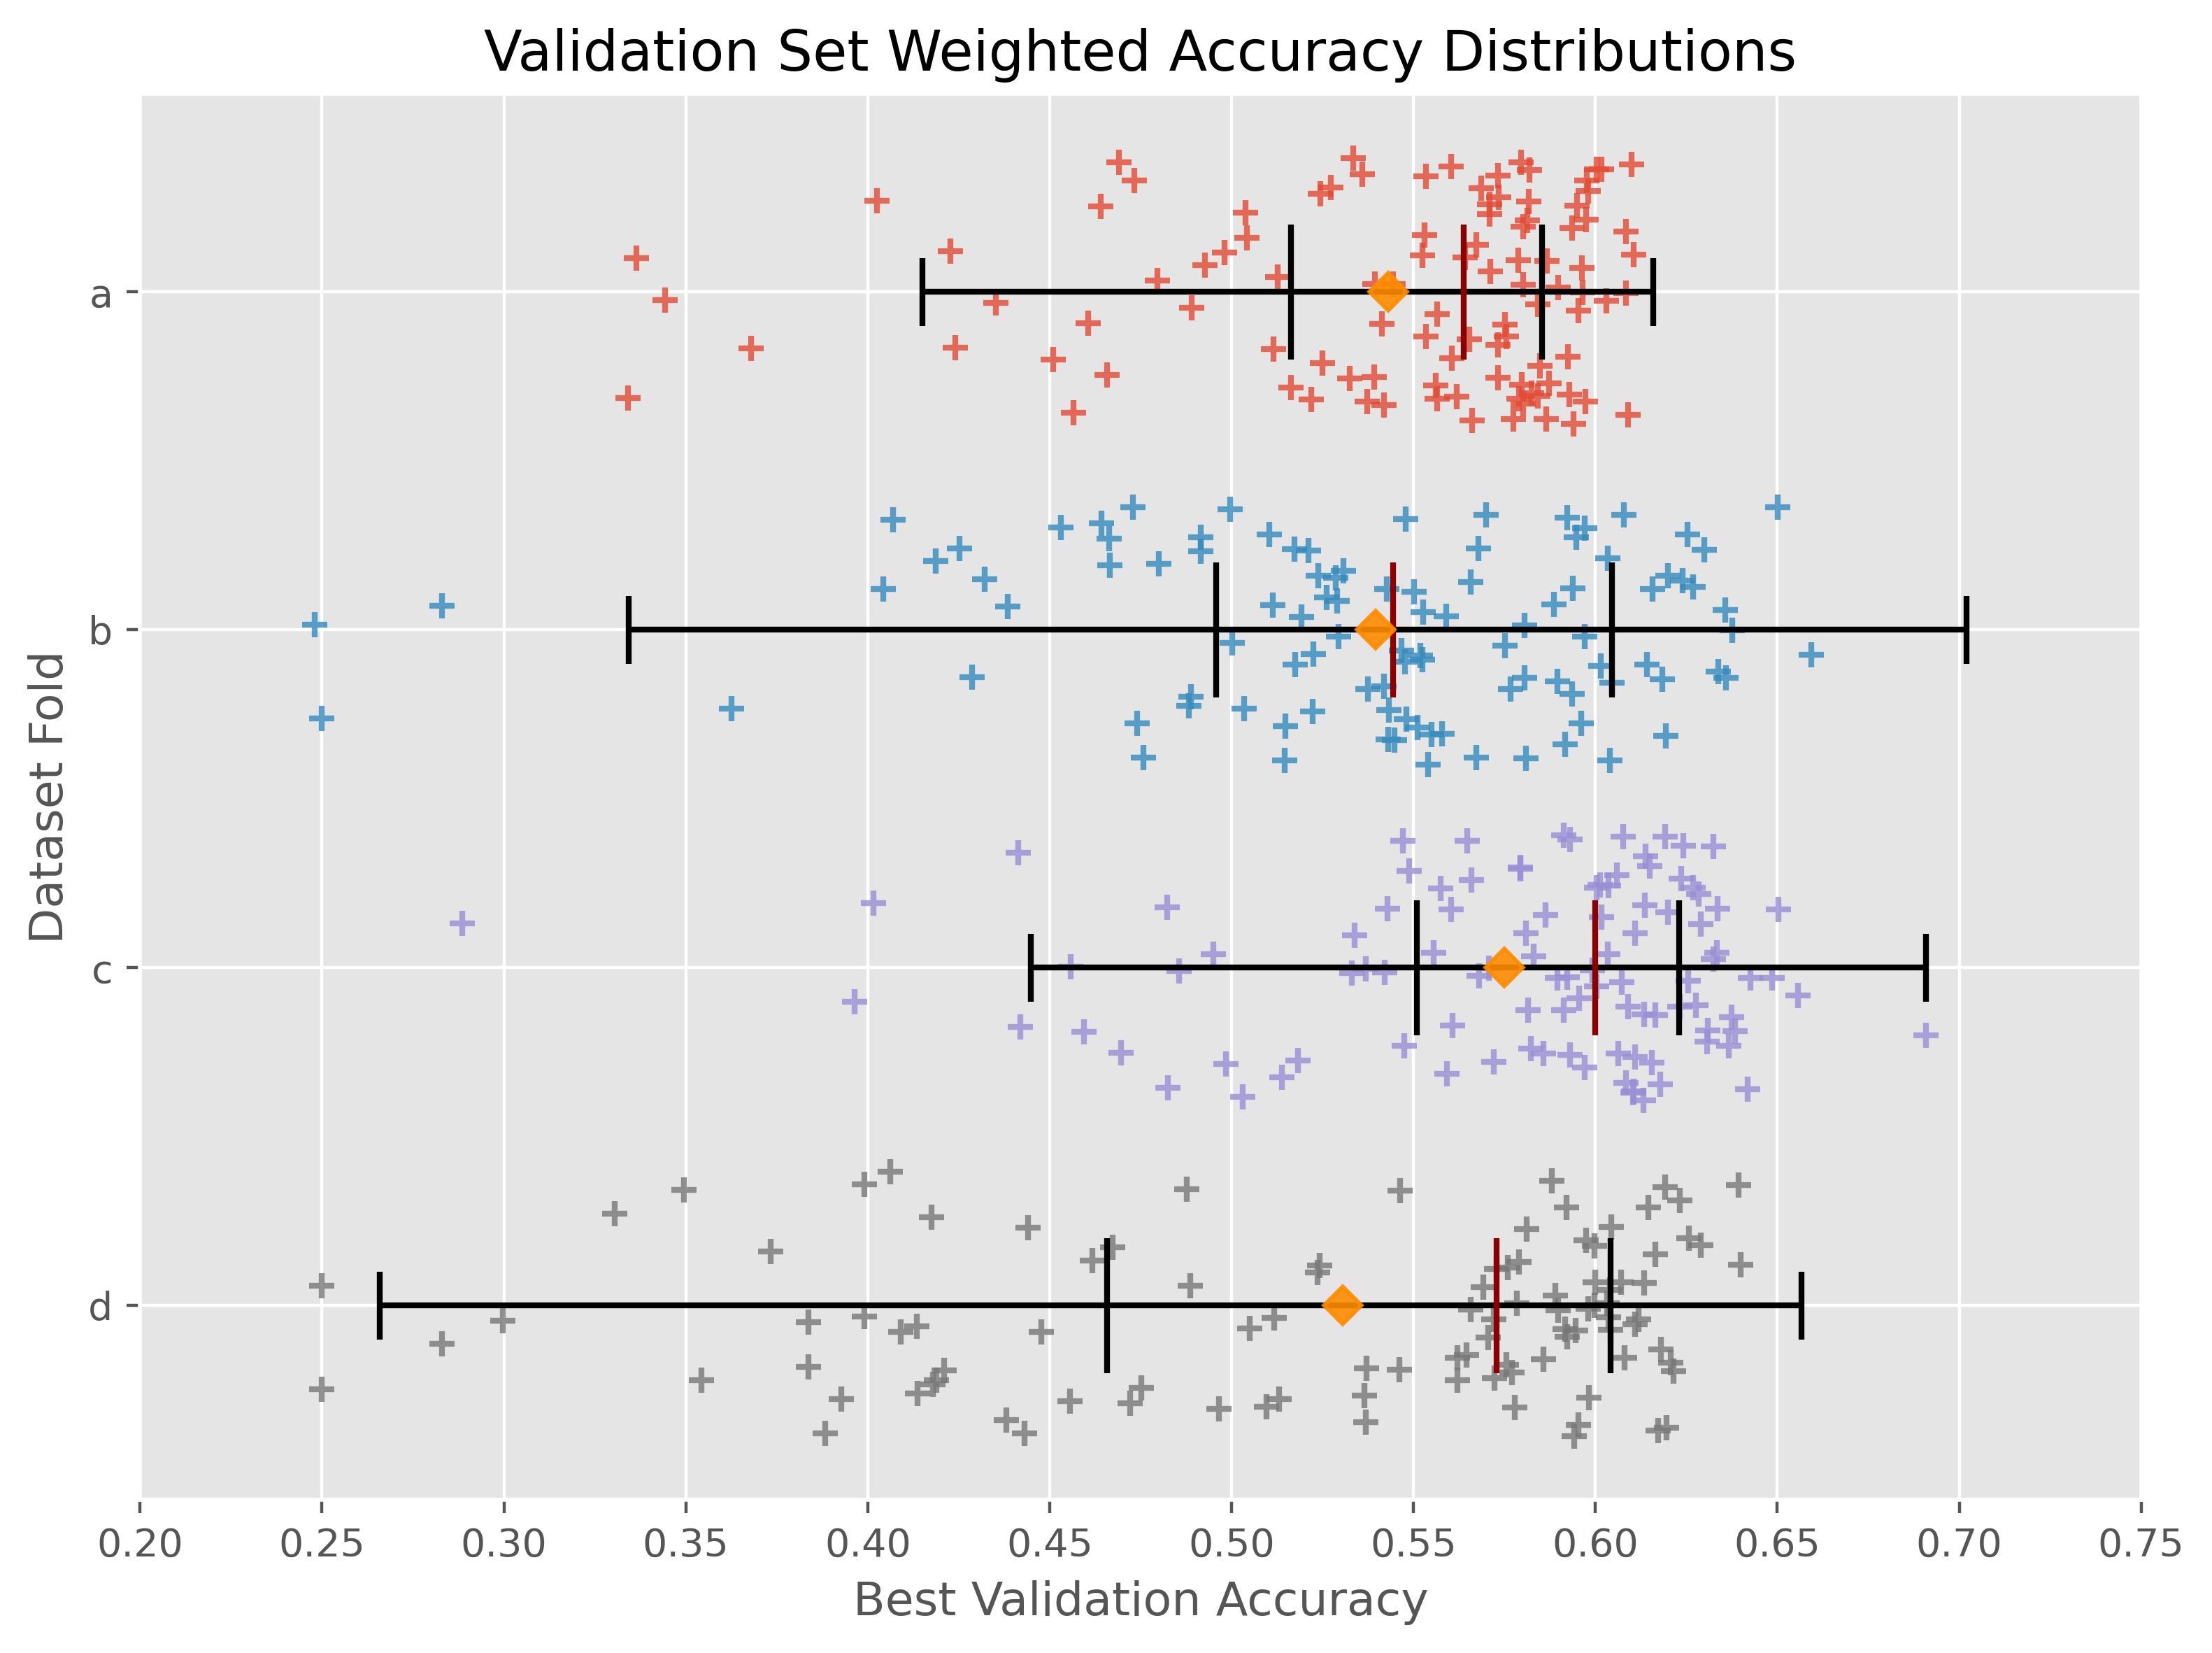
\includegraphics[width=1\textwidth]{Images/best_val_accuracy.png} 
    \caption{Validation set OWA performance of the SCNN models trained on each dataset fold. Ticks are shown at ends of the first and third quartiles, $Q_1$ and $Q_3$, the median (red) and at either $1.5\times$ the inter-quartile range from $Q_1$ and $Q_3$ or the maximum / minimum recorded value, whichever is closest to the median. The mean values are denoted by orange diamonds.} 
    \label{fig:val_fold_boxes}
\end{figure}

\noindent
Because model convergence was still unstable within this tuned hyperparameter range, it was decided to apply an ensemble approach to the SCNN predictions. All models trained on the same fold with validation set OWA scores above the median value in the worst performing fold (taken to be $55\%$) were used to make predictions on the test set. These selected models were combined using a voting approach, where the predicted class with the highest number of votes was selected as the final prediction. The performance of this method for four-class and binary classification in the test set is presented in Tables \ref{table:quad_results_full} and \ref{table:binary_results_full} respectively, along with the performance of the traditional machine learning methods described previously.\\

\noindent
It was hypothesised that label smoothing \cite{xia_towards_2025} could improve model performance by encoding a small amount of uncertainty in the training set labels. Due to the high computational cost of training these full ensemble SCNN models, this was tested only on dataset fold ``a'' (as labelled in Figure \ref{fig:val_fold_boxes}). The test set performance results of these trials are presented in Table \ref{tab:label_smooth_tests}, and show that increasing label smoothing from $0\%$ to $20\%$ slightly reduces OWA scores. It should be noted, however, that these results cannot be used to inform the SCNN method trialled here because they would introduce test-set information into the model. Label smoothing could therefore also be investigated further by future work.

\begin{table}[htbp]
    \centering
    \begin{tabular}{llcccc}
        \toprule
        Smoothing & Metric & Normal & Hyperplastic & Adenoma & Cancer \\
        \midrule
        \multirow{5}{*}{0\%} 
            & Sensitivity          & 0.662 & 0.258 & 0.452 & 0.783 \\
            & Specificity          & 0.708 & 0.762 & 0.936 & 0.972 \\
            & Accuracy             & 0.699 & 0.680 & 0.699 & 0.945 \\
            & False Positive Rate  & 0.292 & 0.238 & 0.064 & 0.028 \\
            & Overall Weighted Accuracy & \multicolumn{4}{c}{0.5387} \\
        \midrule
        \multirow{5}{*}{10\%} 
            & Sensitivity          & 0.643 & 0.257 & 0.458 & 0.782 \\
            & Specificity          & 0.716 & 0.755 & 0.933 & 0.971 \\
            & Accuracy             & 0.702 & 0.674 & 0.700 & 0.944 \\
            & False Positive Rate  & 0.284 & 0.245 & 0.067 & 0.029 \\
            & Overall Weighted Accuracy & \multicolumn{4}{c}{0.5349} \\
        \midrule
        \multirow{5}{*}{20\%} 
            & Sensitivity          & 0.650 & 0.266 & 0.436 & 0.786 \\
            & Specificity          & 0.713 & 0.751 & 0.937 & 0.967 \\
            & Accuracy             & 0.700 & 0.672 & 0.692 & 0.941 \\
            & False Positive Rate  & 0.287 & 0.249 & 0.063 & 0.033 \\
            & Overall Weighted Accuracy & \multicolumn{4}{c}{0.5345} \\
        \bottomrule
    \end{tabular}
    \caption{Fold ``a'' test-set SCNN classification performance with a 55 \% voting threshold
    and different label-smoothing levels.}
    \label{tab:label_smooth_tests}
\end{table}

\subsection{SCNN Performance Investigation}
\begin{figure}[htbp]
    \centering
    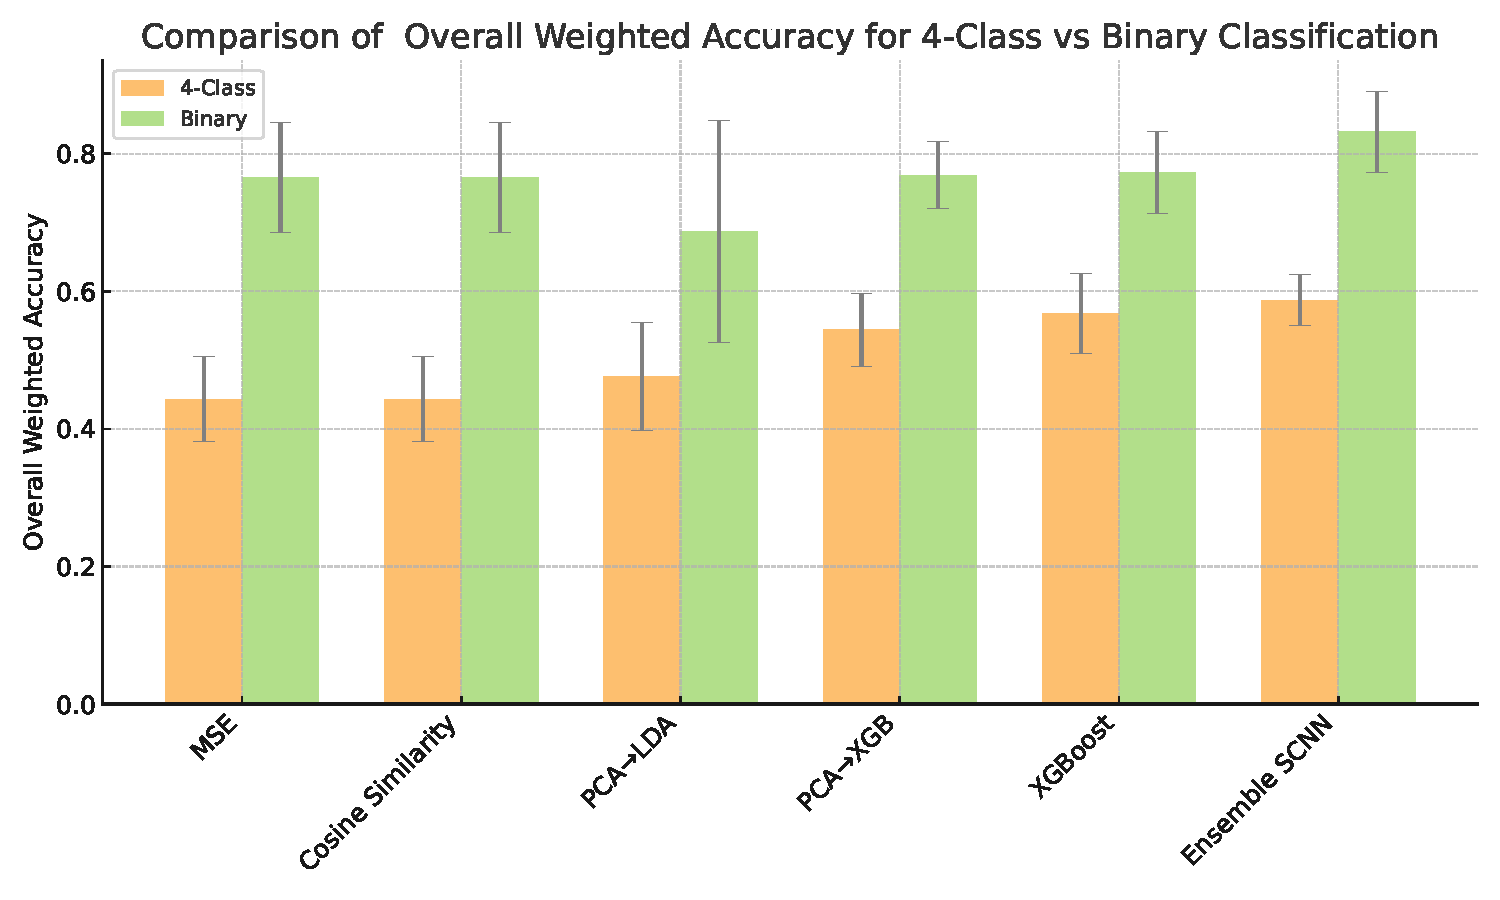
\includegraphics[width=0.8\textwidth]{Images/combined_accuracy.pdf}
    \caption{The OWA achieved by each ML method, and the SCNN method both for binary and four-class classification. The SCNN method is seen to perform best in both cases.}
    \label{fig:combined_accuracy}
\end{figure}

The performance of the SCNN method beats all other methods in both binary and four-class classification, as shown in Figure \ref{fig:combined_accuracy}, achieving weighted overall accuracies of $0.832\pm0.059$ and $0.587\pm0.037$ respectively. I therefore investigated the ensemble SCNN predictions further to discover the strengths and weaknesses of this model. The summed confusion matrix for four-class classification across the four folds is shown in Table \ref{tab:confusion_SCNN_4class}. From this, we see that the model is best at classifying normal and cancerous tissue, but predicts hyperplastic tissue to be normal more often than not. It also frequently predicts adenomatous tissue to be normal or cancerous. These results, however, are somewhat expected and in fact desired given the sample classification method used (§\ref{sec:mdethods:data_collection}). This implies there is a limit to the usefulness of the comparative metrics. I therefore also conducted qualitative analysis with the assistance of Dr. Nalalla from the University of Exeter. Some of the SCNN predictions analysed are presented in Figure \ref{fig:categorisation_train_test}. Here, we see that the model refuses to fit to some samples within the training set (Figure \ref{fig:categorisation_train_test}.c), strongly indicating that the model is learning to classify pixels better than the classifications it is provided with to train.\\

\noindent
To further demonstrate how this performance is superior to that suggested by the classification statistics, we can compare the H\&E images in Figure \ref{fig:IR_and_HE_categories}.i-iv with the SCNN predictions in Figure \ref{fig:categorisation_train_test}.i-iv. For the sample presented in the i) subplots, we see that the SCNN model has predicted some normal tissue to be hyperplastic, and some to be cancerous. This is thought to be due to the presence of inflamed tissue in the sample, which is best described as an additional classification category. The sample presented in the iii) subplots clearly shows how the model has learnt to correctly differentiate between adenomatous and normal tissue. Furthermore, the predictions of hyperplasticity in the iv) subplots are thought to be due to the presence of necrotic tissue in the sample, which again is best described as an additional classification category. Future work could therefore investigate the application of this model to more finely labelled datasets, or could try incorporating more samples in the training set to provide labelled information on inflamed and necrotic regions. \\

\noindent
To complement this analysis, I also investigated the confidence the model has in its predictions by evaluating the number of votes each class receives in the ensemble prediction for the same pixel. The results of this analysis for the same samples as were previously discussed are presented in Figure \ref{fig:uncertainty}. In Figure \ref{fig:uncertainty}.iv, we see that the model is particularly uncertain around the transition from cancerous to hyperplastic predictions. This is expected, as such regions are unlikely to have sharp boundaries. Furthermore, in Figure \ref{fig:uncertainty}.iii, we see that it is less confident in predicting tissue to be normal than adenomatous, which is again likely due to diffuse boundaries which should really be considered as containing cells intermediate to either classification.

\begin{table}[h]
\centering
\begin{tabular}{l|rrrr}
Labelled $\backslash$ Predicted & Normal & Hyperplastic & Adenoma & Cancer \\ \hline
Normal        & 164993 &  28191 &  31533 &   7890 \\
Hyperplastic  &  77386 &  62551 &  29068 &  23767 \\
Adenoma       & 124631 &  69665 & 330515 &  68378 \\
Cancer        &   9588 &  14258 &  17966 & 132174 \\
\end{tabular}
\caption{Summed confusion matrix  (rows = true class, columns = predicted class).}
\label{tab:confusion_SCNN_4class}
\end{table}

\begin{figure}[htbp] 
    \centering 
    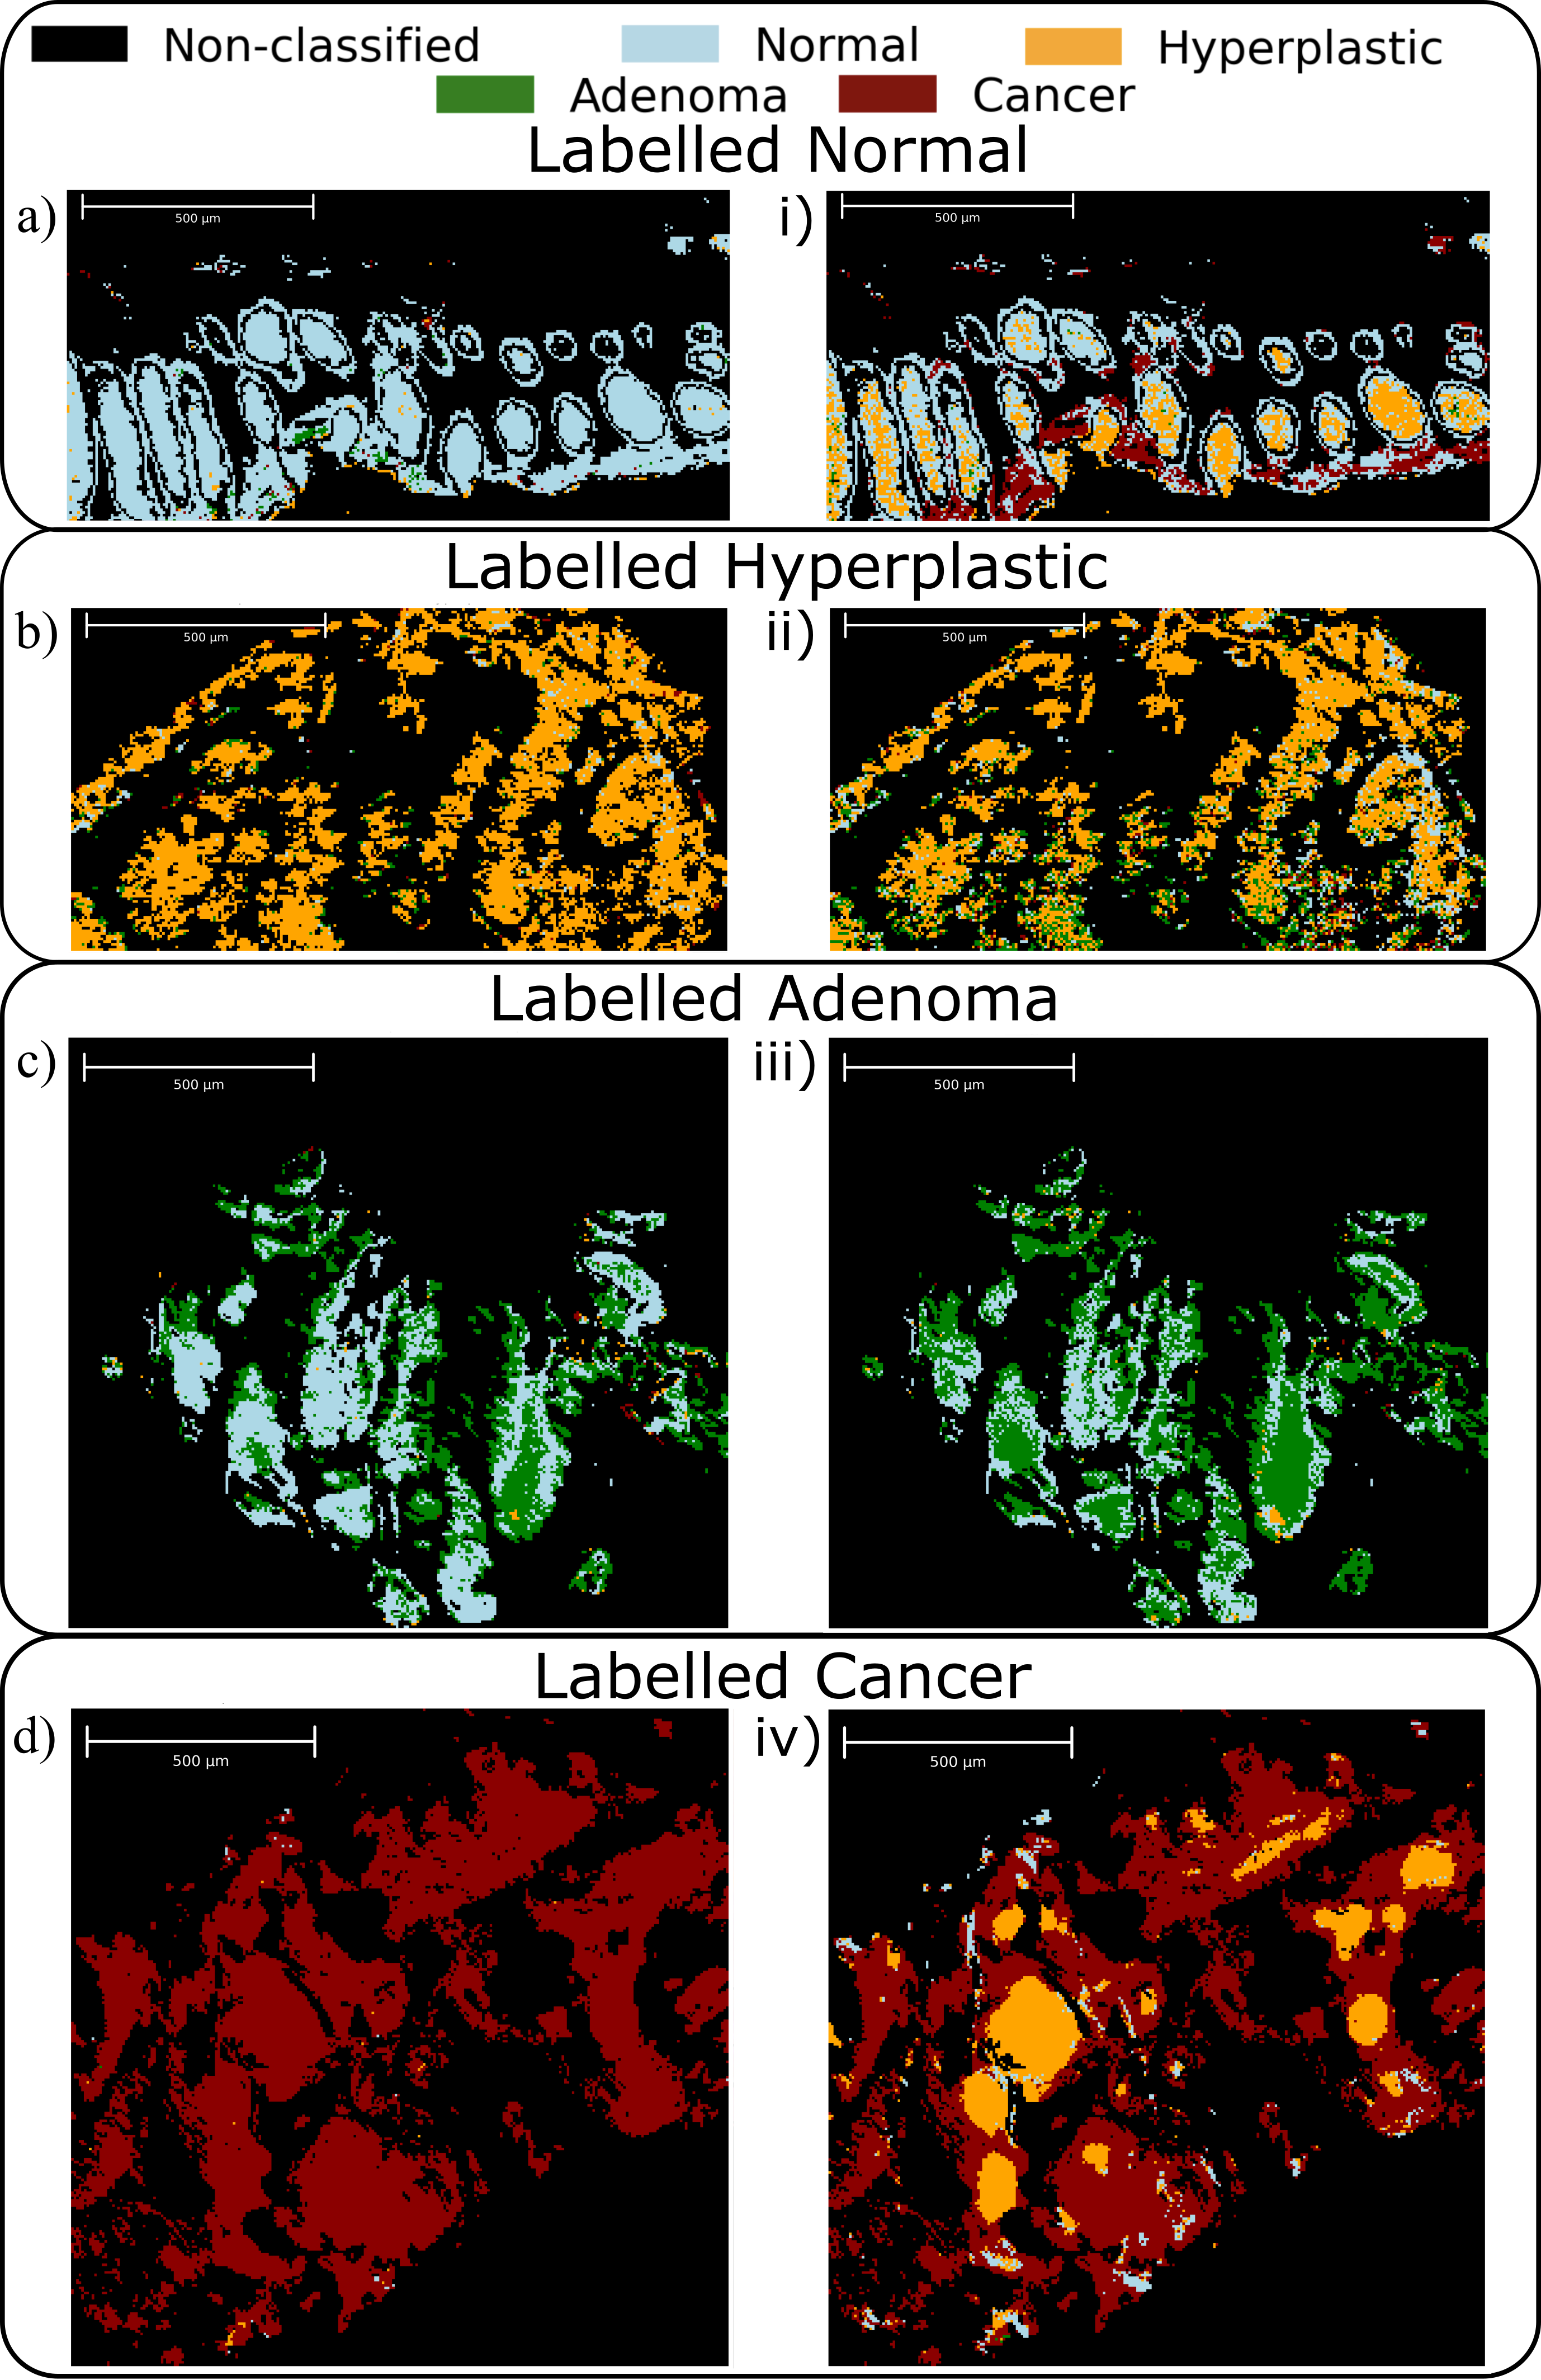
\includegraphics[width=0.8\textwidth]{Images/Categorisation_train_test.png} 
    \caption{SCNN classification predictions for the same samples when each is used in the training set (a-d) and when each is used in the test set (i-iv).} 
    \label{fig:categorisation_train_test} 
\end{figure}

\begin{figure}[htbp] 
    \centering 
    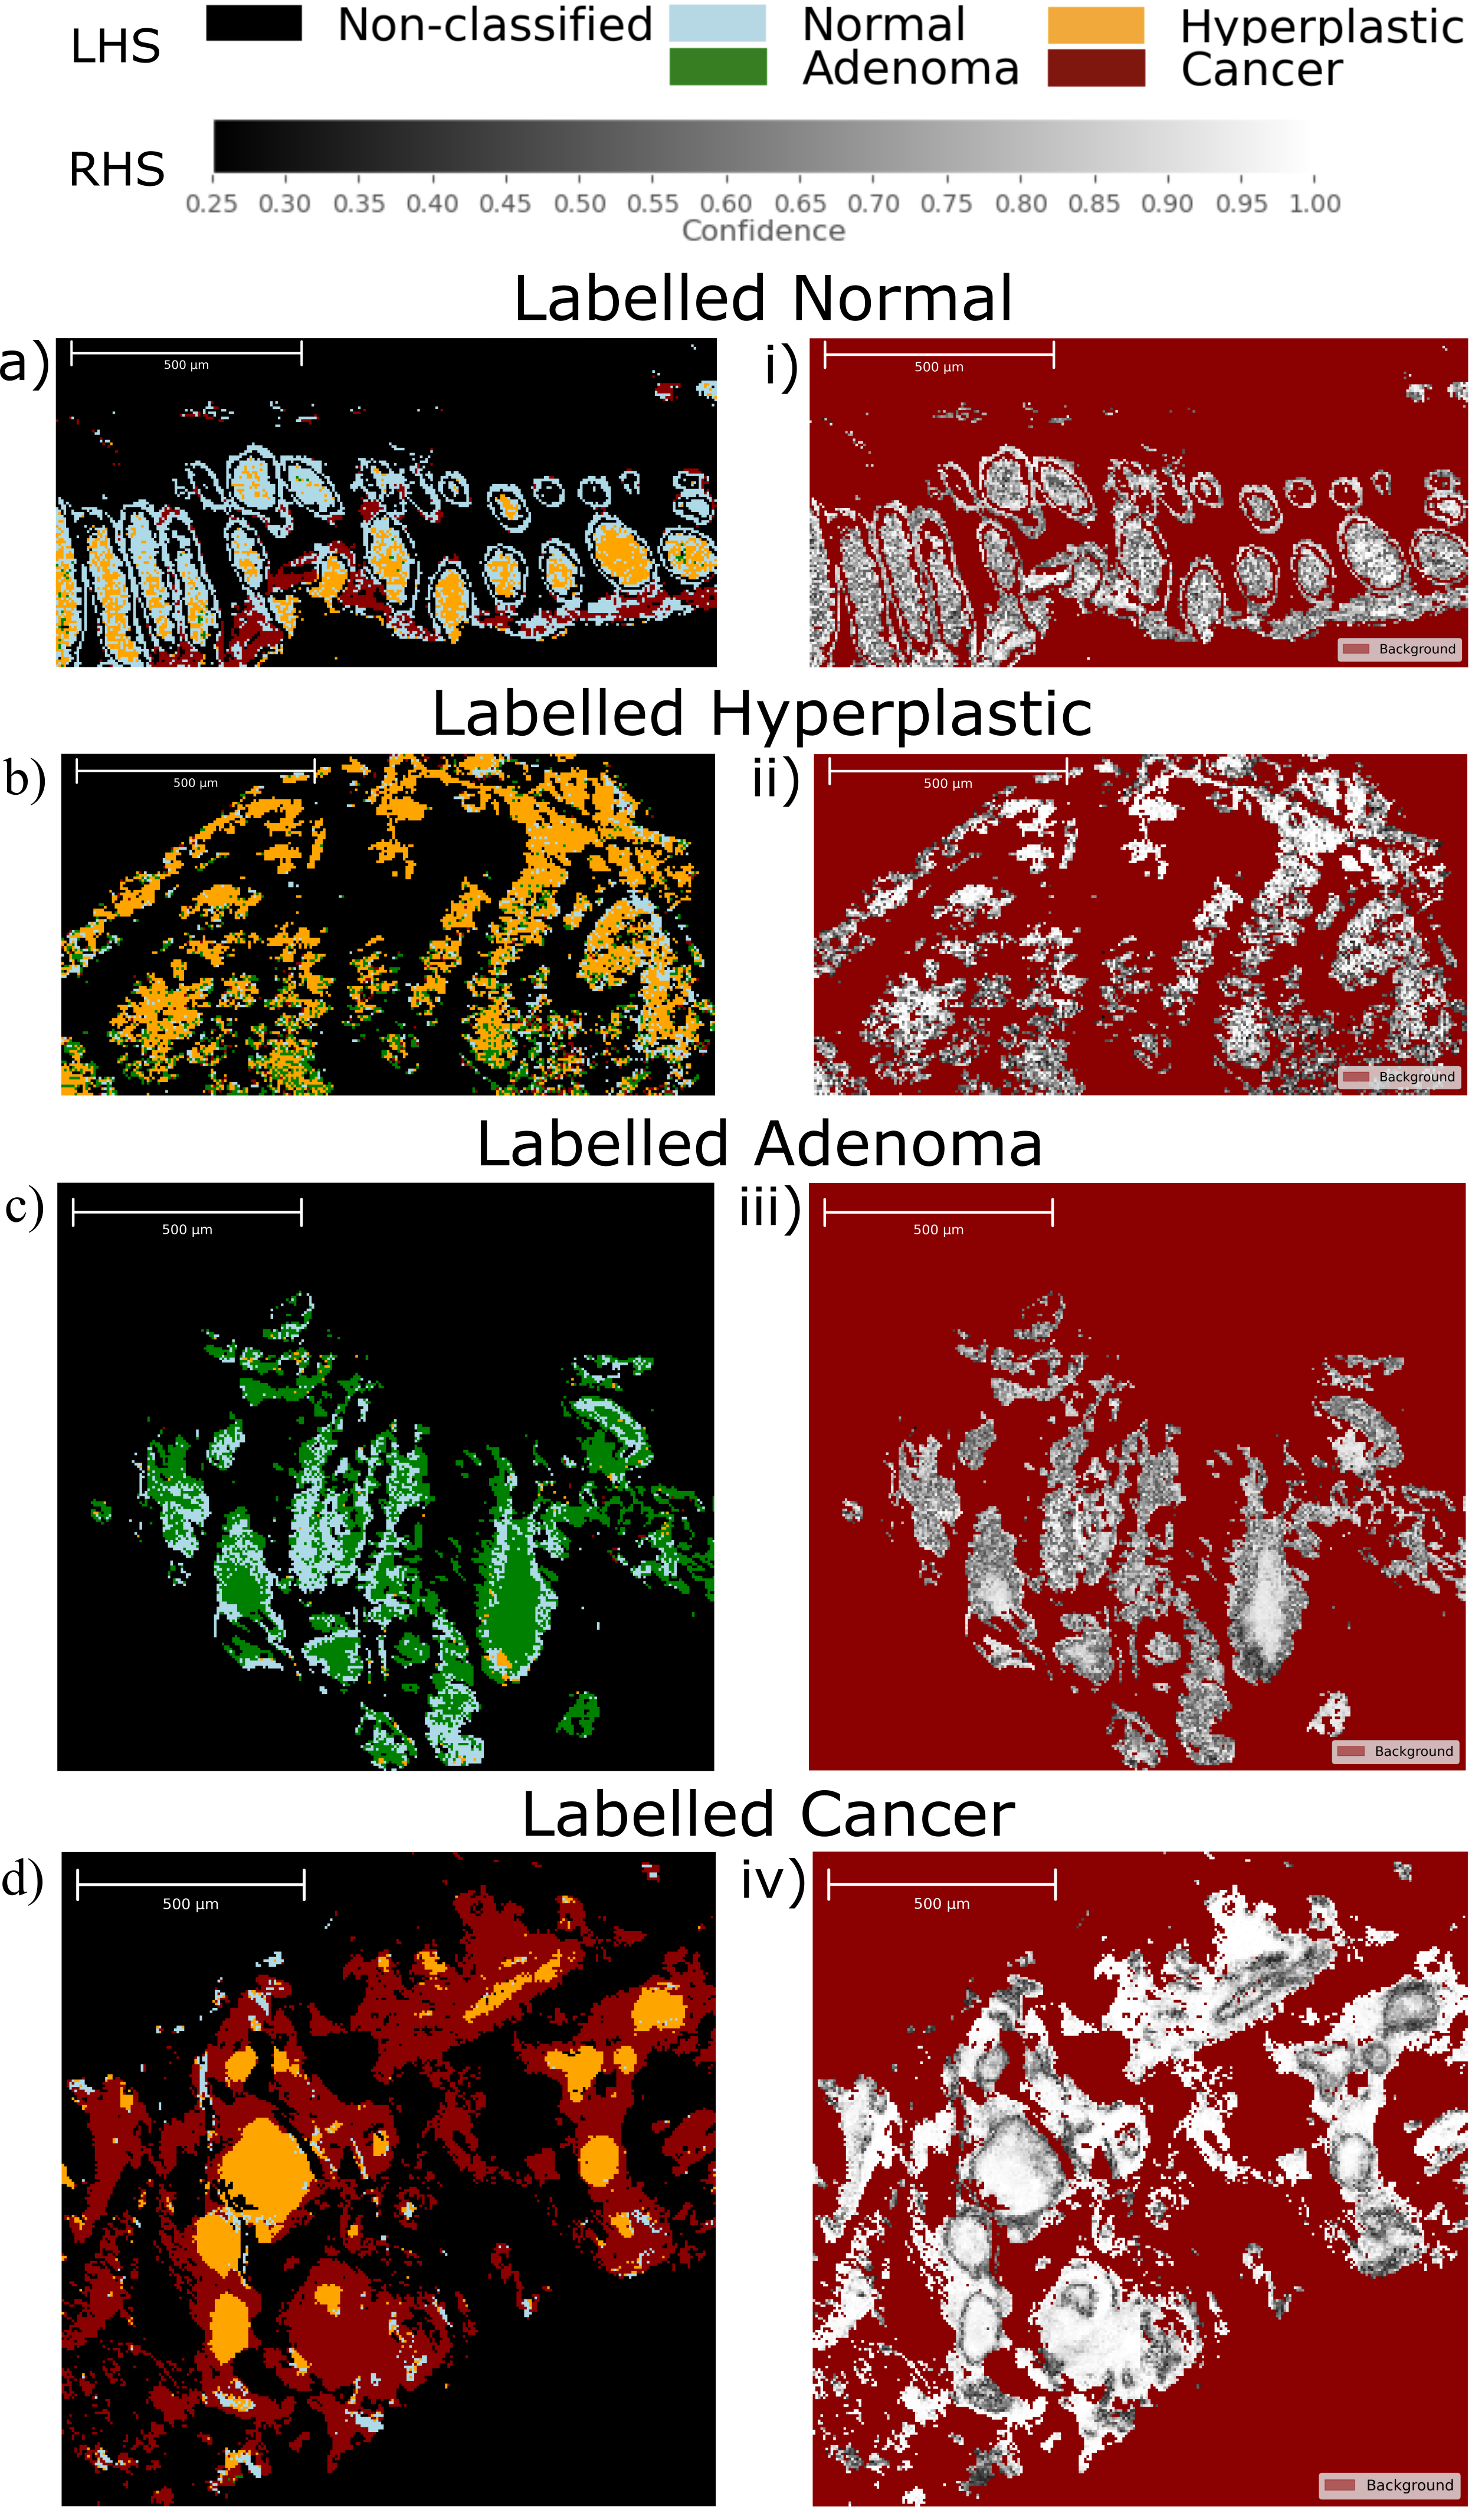
\includegraphics[width=0.8\textwidth]{Images/Confidence.png} 
    \caption{The confidence of the SCNN model in its classification predictions for each sample considered in Figures \ref{fig:IR_and_HE_categories} and \ref{fig:categorisation_train_test}.} 
    \label{fig:uncertainty}
\end{figure}

\subsubsection{LIME Explanations}
\label{sec:lime_explanations}
LIME analysis was also conducted on a subset of the SCNN validation set predictions - 5000 pixels per classification type (grouped by their training label). This allowed for the generation of importance weightings for each wavenumber and prediction classification. These can be seen in Figure \ref{fig:lime_weights_classes}. These results indicate that the region from $1000$-$1200$ cm$^{-1}$ is particularly relevant for all classifications, and that the region from $1460$-$1560$ cm$^{-1}$ is much less important. This could be used to help guide the development of next generation imaging methods such as those being developed as part of the TROPHY project \cite{noauthor_ultrafast_2022}.

\begin{figure}[htbp]
    \centering
    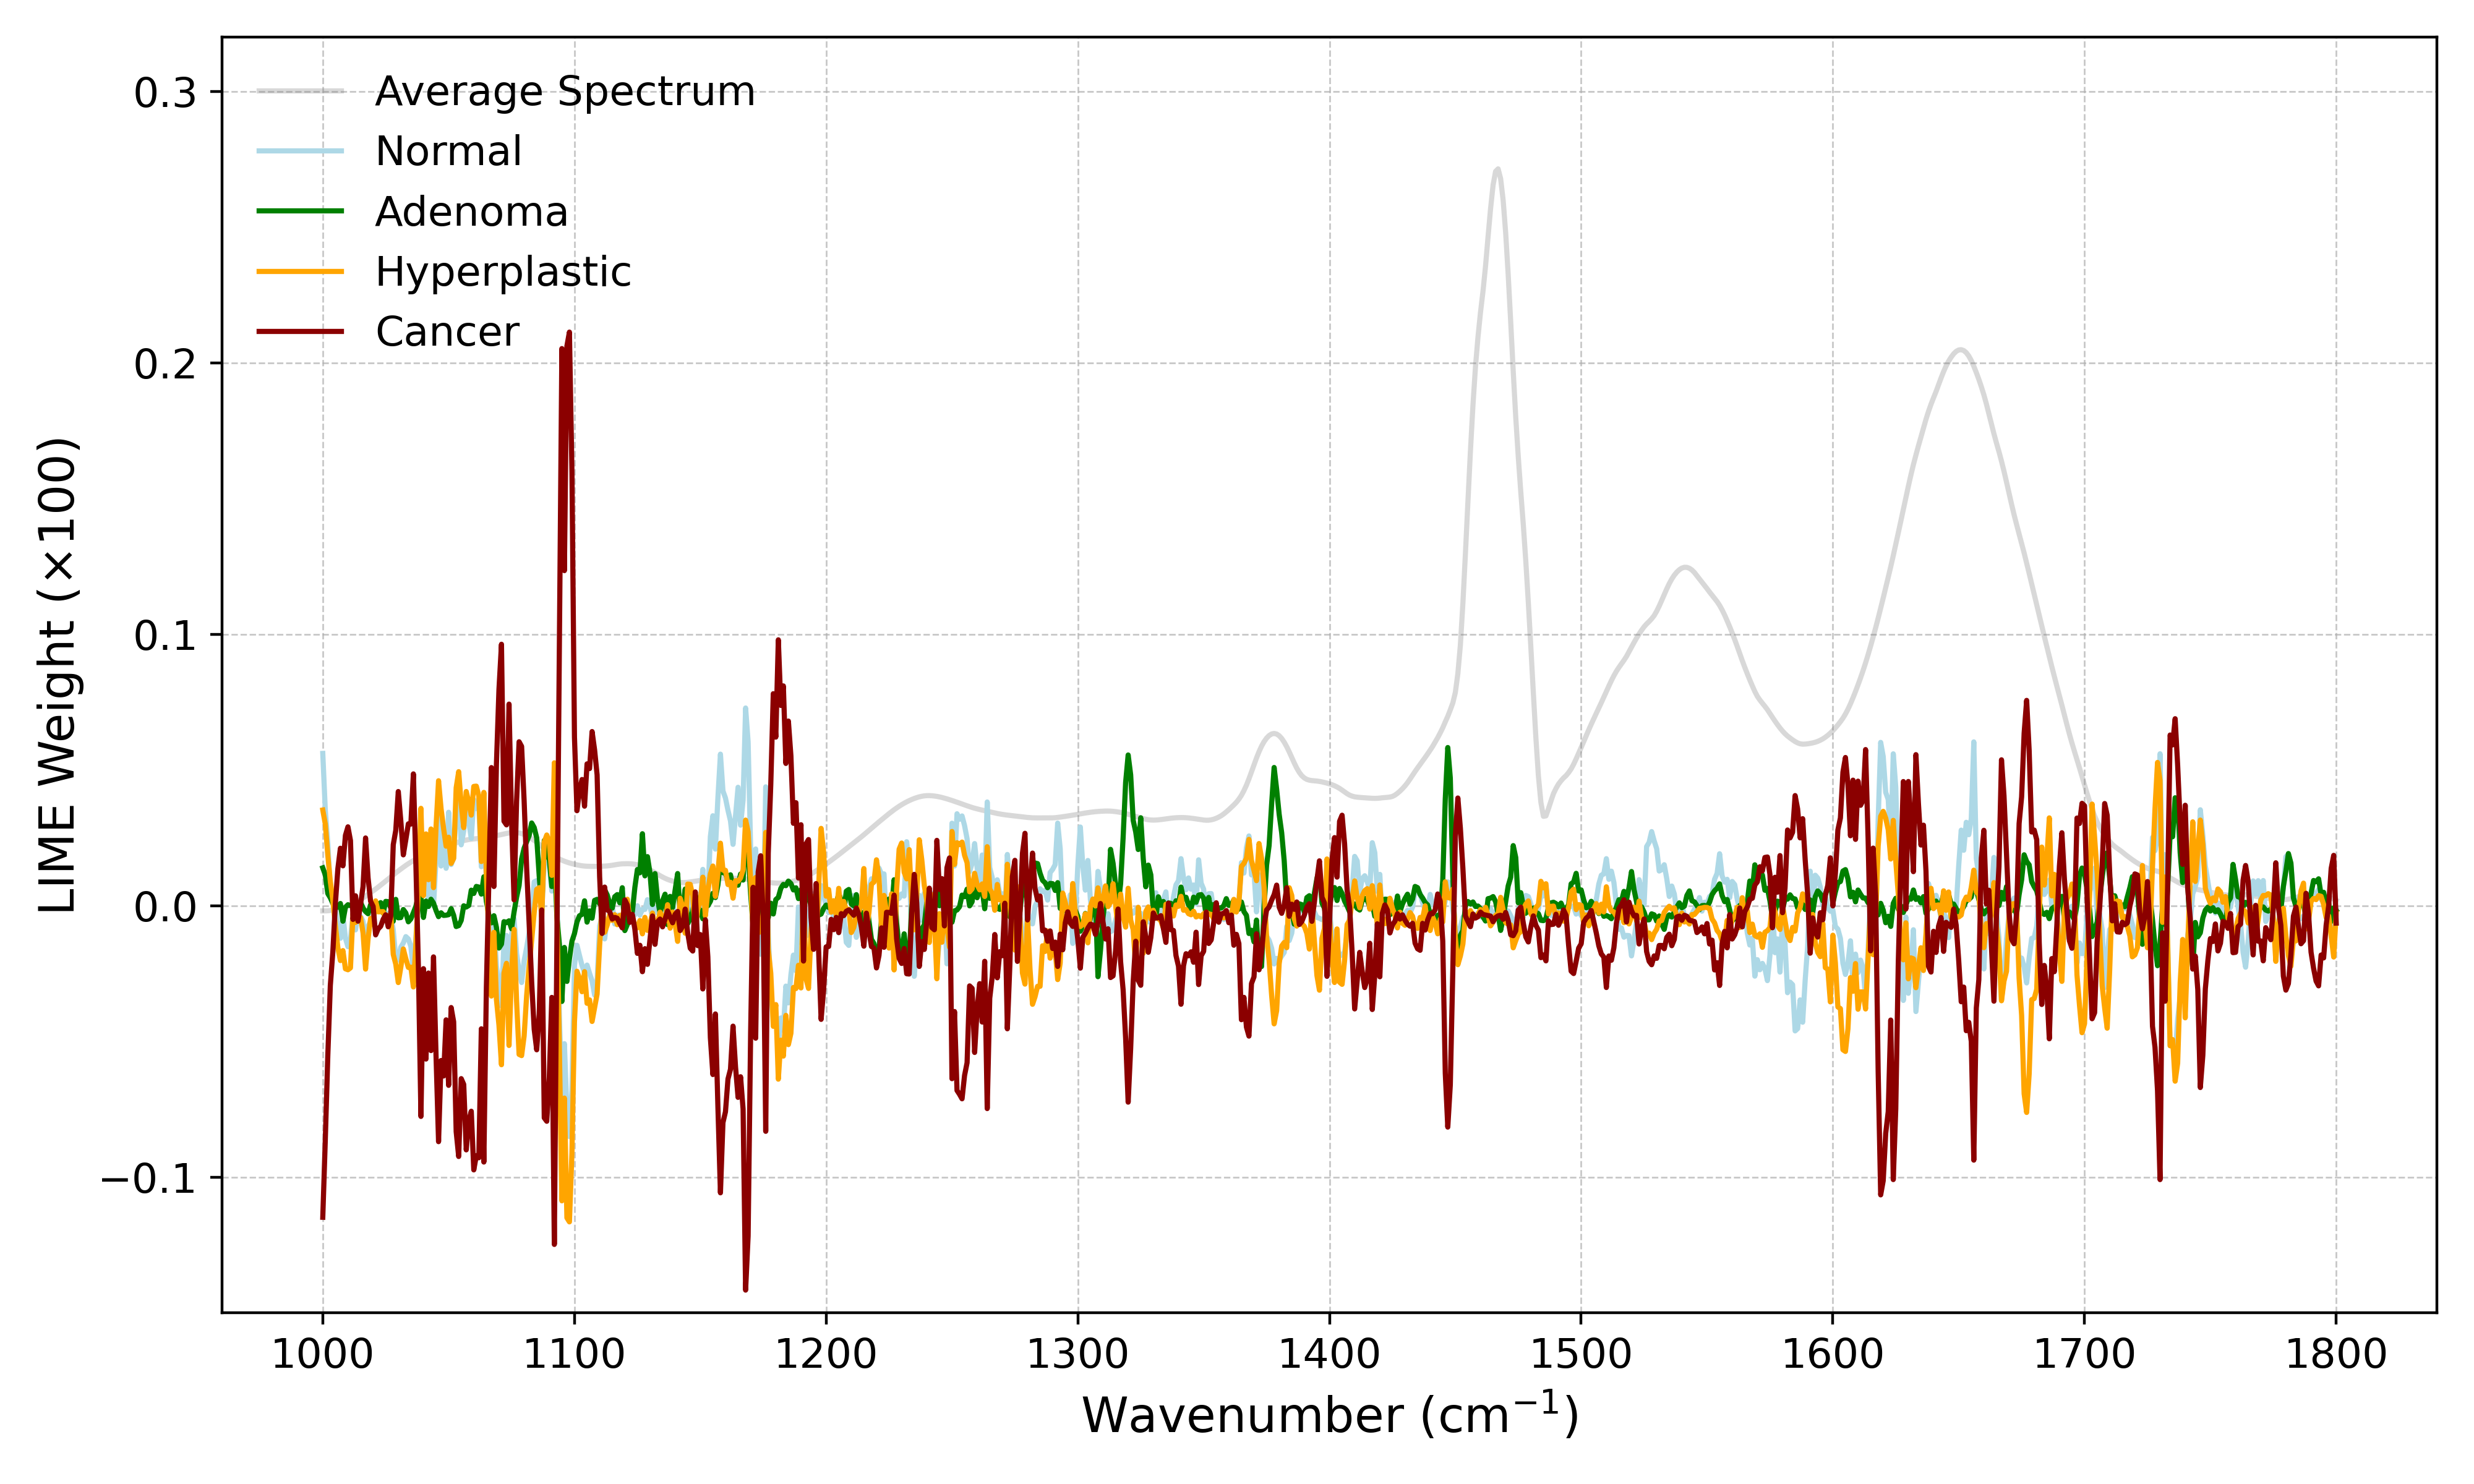
\includegraphics[width=0.8\textwidth]{Images/lime_contributions_plot.png}
    \caption{LIME analysis results showing the average LIME importance associated with each wavenumber feature.}
    \label{fig:lime_weights_classes}
\end{figure}

\subsection{CRIME Analysis}
The LIME explanations found in the previous section enable the generation of explanations for any individual prediction. However, they do not provide a good understanding of how the model works as a whole. To address this, the CRIME method described in §\ref{sec:methods:crime} was applied using the $20,000$ pixel explanations generated for §\ref{sec:lime_explanations}. For this, each VAE network was trained on the validation set pixels. Throughout this training, the $\alpha$ and $\beta$ hyperparameters were tuned such as to generate distinct clusterings in latent space. These hyperparameters used were $\alpha=1000$, $\beta=0.1$ for the CP and DT VAEs, and $\alpha=1000$, $\beta=1\times10^{-3}$ for the CT VAE. The contexts were then formed by K-means clustering with $K=100$ in all cases. An example latent space representation and its associated contexts for $K=20$ produced by the unsupervised CP VAE is shown in Figure \ref{fig:latent_space}. This demonstrates how the LIME explanations can be used to effectively separate tissue classifications in latent space.\\

\noindent
To quantify this separability, I calculated the SCNN ensemble prediction associated with each explanation. For each context, I then counted the number of these predictions associated with each tissue classification. The same was done using the training label associated with each explanation. In the $K=100$ case applied to the latent space representation found in Figure \ref{fig:latent_space}.b, this generated the histograms shown in Figure \ref{fig:crime_groupings}. A careful analysis of these histograms shows that the cancer dominated contexts are associated with very few non-cancer predictions, and the same is also true for all of the dominant peaks in the other classifications. I therefore hypothesise that this method has found some independent mappings from explanations into tissue classifications. To investigate this further, I classified each context according to the majority SCNN ensemble classification associated with the explanations within that context. By then finding the average spectra and LIME weightings associated with each context, I was able to form multiple explained spectra for each classification. Figure \ref{fig:crime_lime_plots} shows a few examples of these explained context spectra for the same setup as in Figures \ref{fig:crime_groupings} and \ref{fig:latent_space}. Here, we see that although the average spectra for all contexts are similar, the LIME weightings are visibly different, indicating that the model is using different spectral features to make predictions in each context. Further work could therefore be done to investigate the biological and physical significance of these context importance weightings - a task which is feasible, unlike trying to interpret the LIME weightings for each explanation individually.

\begin{figure}[htbp]
  \centering
  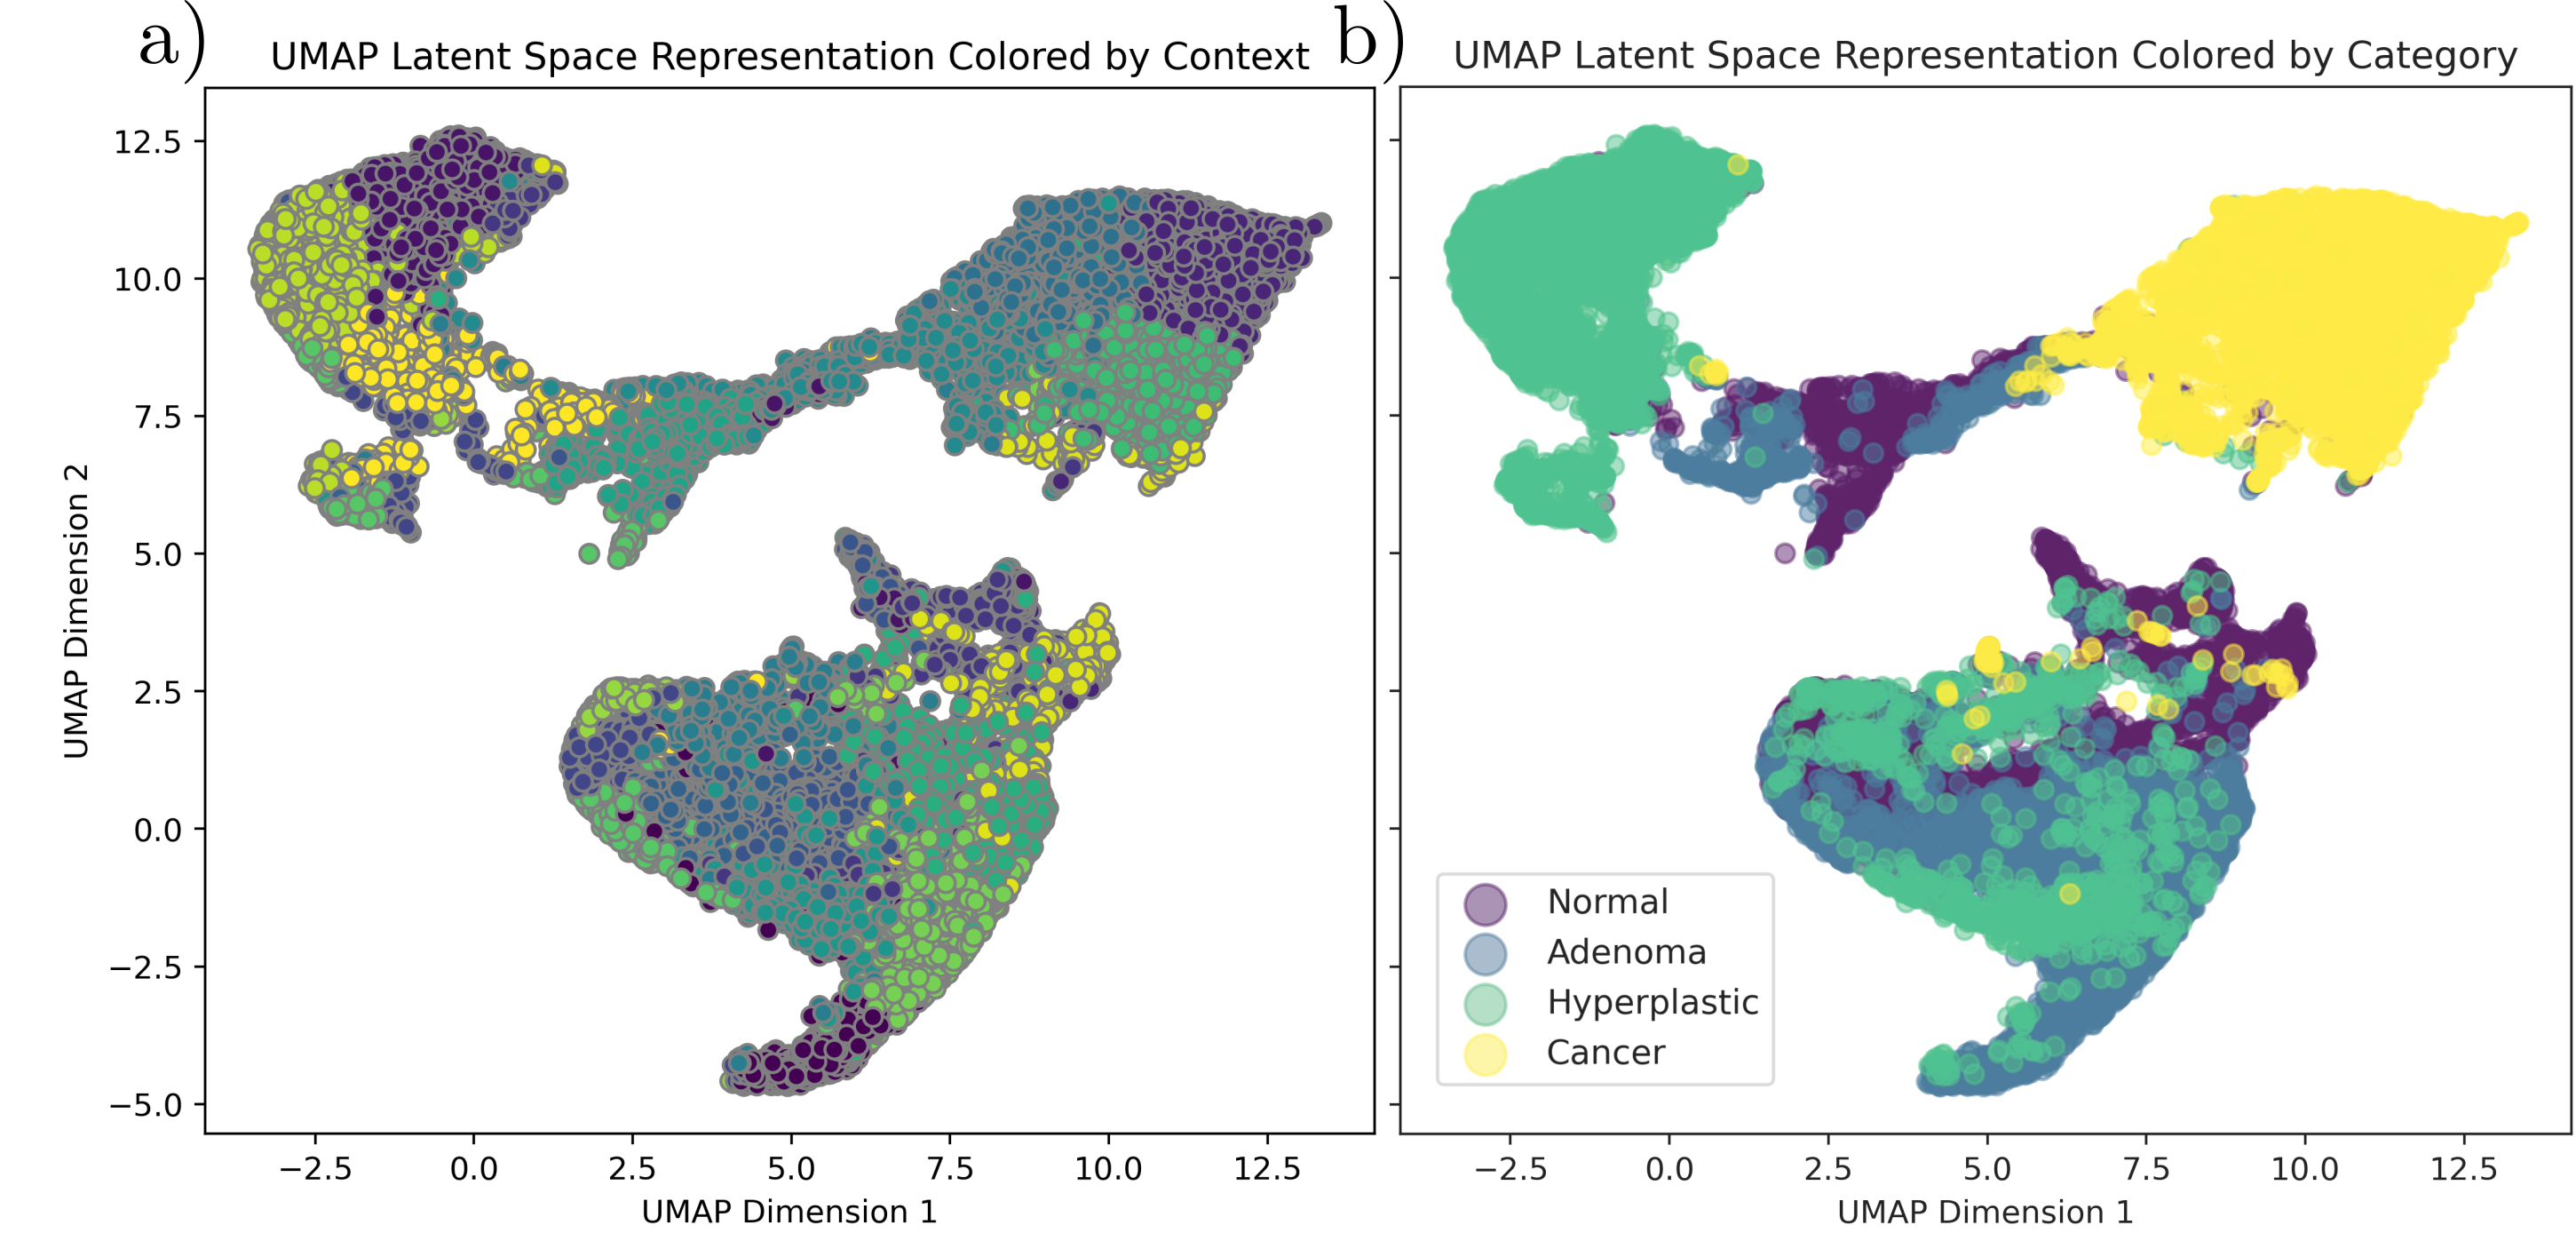
\includegraphics[width=1\textwidth]{Images/crime_umap_h.png}
  \caption{Section a) shows the latent space representation of the LIME explanations generated using the CP VAE. Each colour denotes a different context designated by K-means clustering. Section b) shows the training label associated with each explanation projected into latent space.}
  \label{fig:latent_space}
\end{figure}

\begin{figure}[htbp]
  \centering
  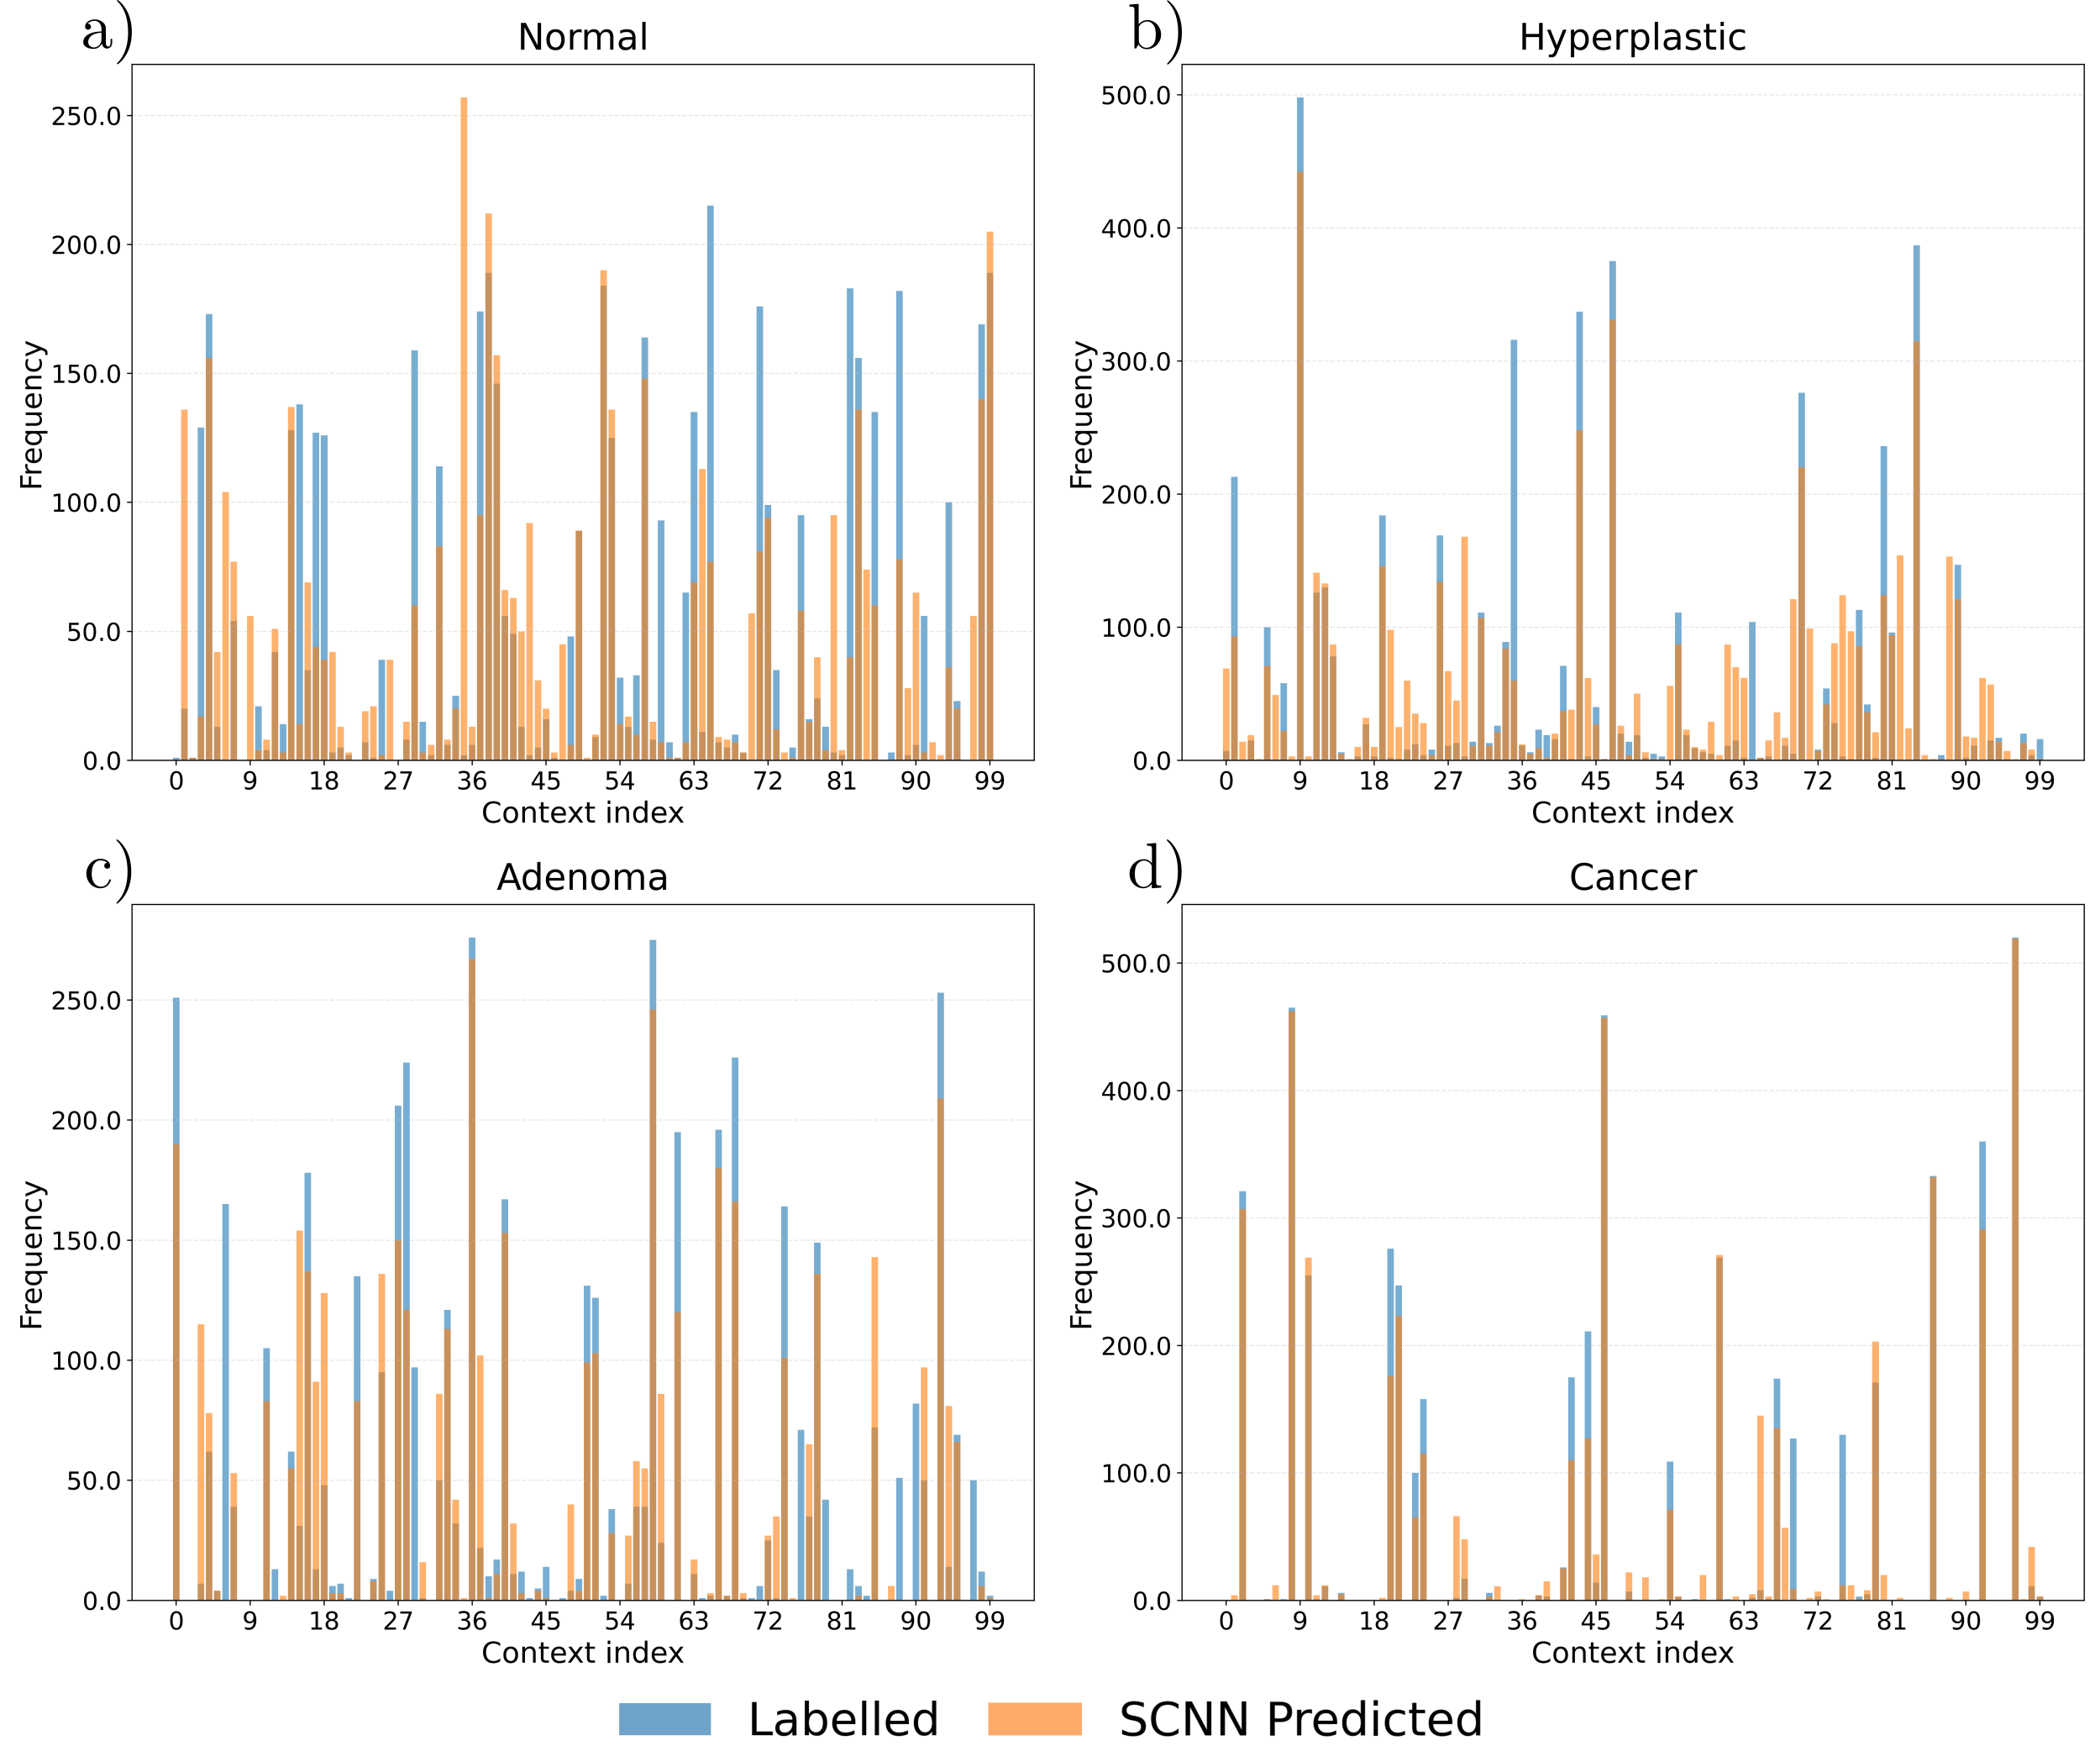
\includegraphics[width=0.8\textwidth]{Images/crime_groupings_by_category_100.png}
  \caption{The number of explanations grouped into each context with associated training labels and SCNN predictions a) normal, b) hyperplastic, c) adenomatous and d) cancerous.}
  \label{fig:crime_groupings}
\end{figure}

\newpage
\begin{figure}[htbp] 
    \centering 
    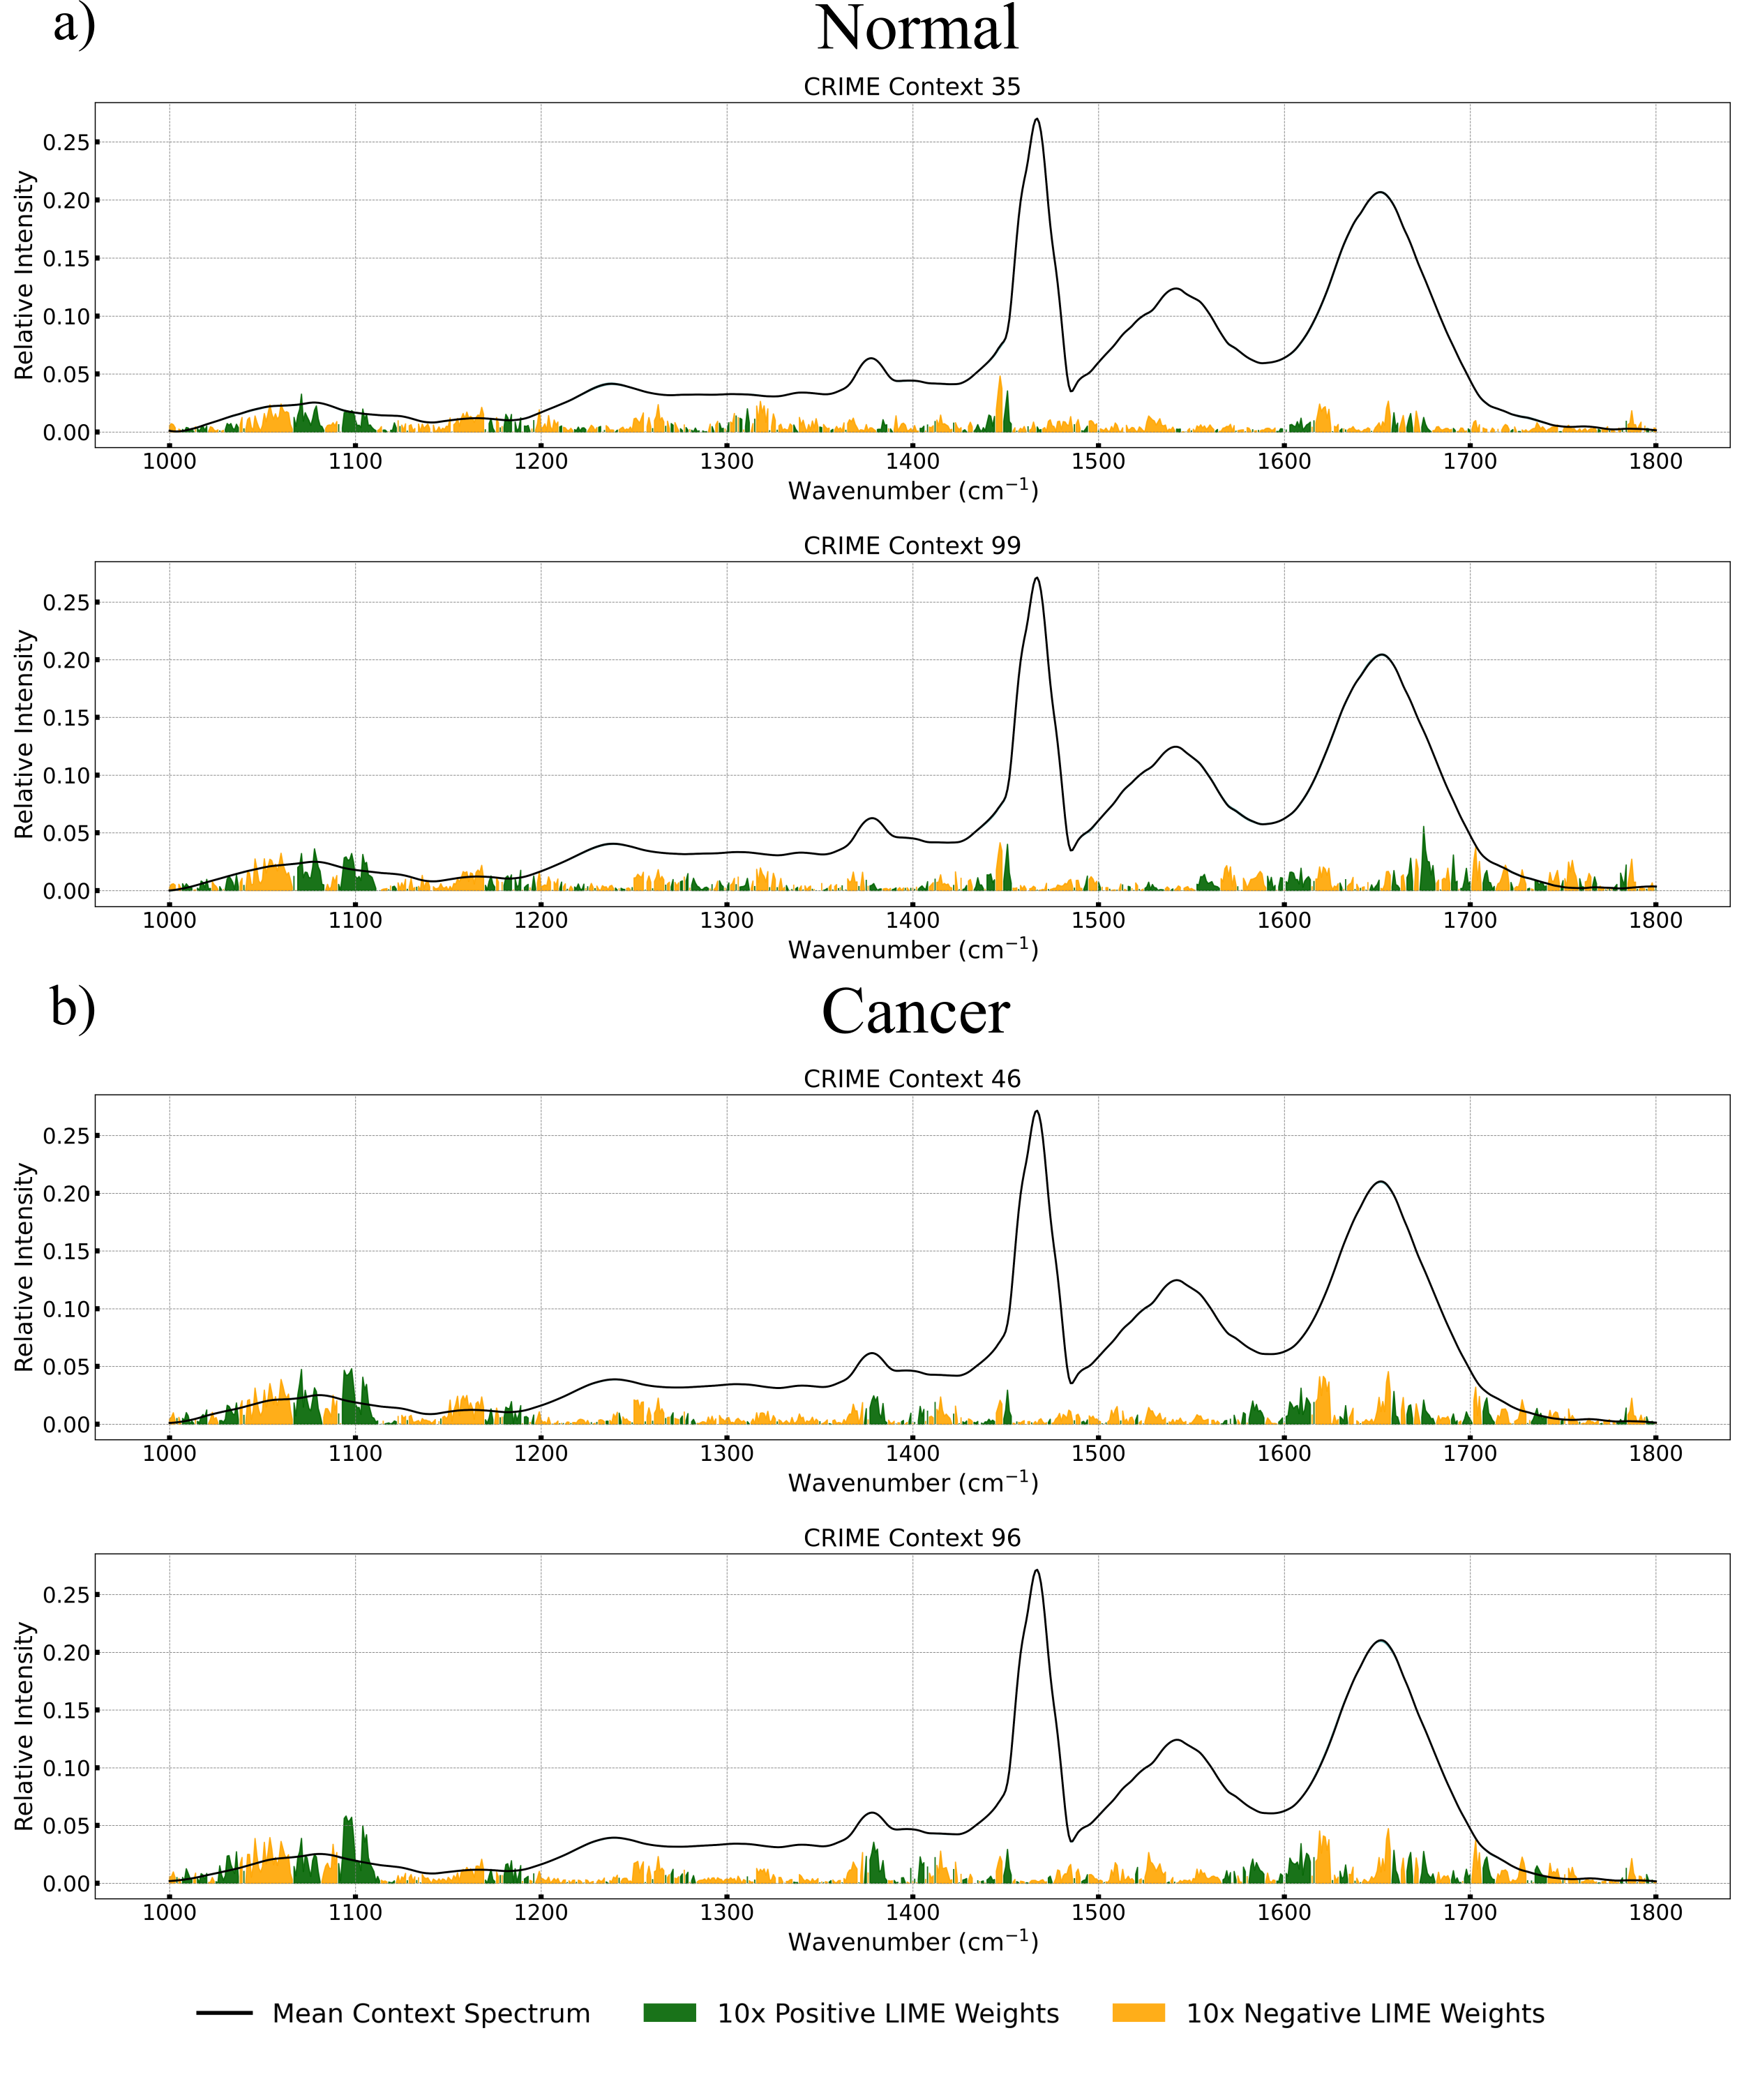
\includegraphics[width=1\textwidth]{Images/crime_lime_plots.png} 
    \caption{CRIME context average spectra and LIME weightings demonstrating the ability of the CRIME method to extract multiple different context environments per classification type.}
    \label{fig:crime_lime_plots} 
\end{figure}

\subsubsection{CRIME Predictions}
The CRIME linear prediction method (LCRIME) described in §\ref{sec:crime_linear} was then employed using the majority classified context spectra and weightings. It was noted, however, that although the CRIME method with an unsupervised CP VAE is able to separate cancer and hyperplastic tissues well, many contexts have multiple similarly-frequent classifications present. To improve this, the M2 semi-supervised versions of the VAEs described in Table \ref{tab:ssvae_arch} were also implemented to encourage the latent space to be more separable. The resulting four-class and binary classification prediction performance metrics achieved by each VAE model are described in full in Tables \ref{tab:quad_results_full_context} and \ref{tab:binary_results_full_context} respectively. Of these, the best metrics for comparison are shown graphically in Figures \ref{fig:quad_context} and \ref{fig:bin_context} for four-class and binary classification tasks respectively. These results show that the LCRIME method generally performs worse than all other methods tested at training-label prediction. The best LCRIME models (CP-0.2 and CT-0.2) are, however, able to reconstruct the model four-class classification predictions better than the MSE and cosine similarity classification are able to reproduce the training labels. LCRIME also achieves a similar performance to the PCA$\to$LDA method by this metric. LCRIME is, however, always out-performed by the PCA$\to$XGB, XGB and ensemble SCNN methods. Despite this, LCRIME still offers advantages because it is intrinsically interpretable and the method by which it makes prediction is easy to explain to patients and clinicians.\\ 

\noindent
Future work could investigate the use of the LCRIME method on less-noisy datasets, or could try to perform more thorough hyperparameter searching by folding the dataset differently. It would also be informative to compare the performance of this LCRIME method against a directly learnt linear mapping model.

\begin{figure}
    \centering 
    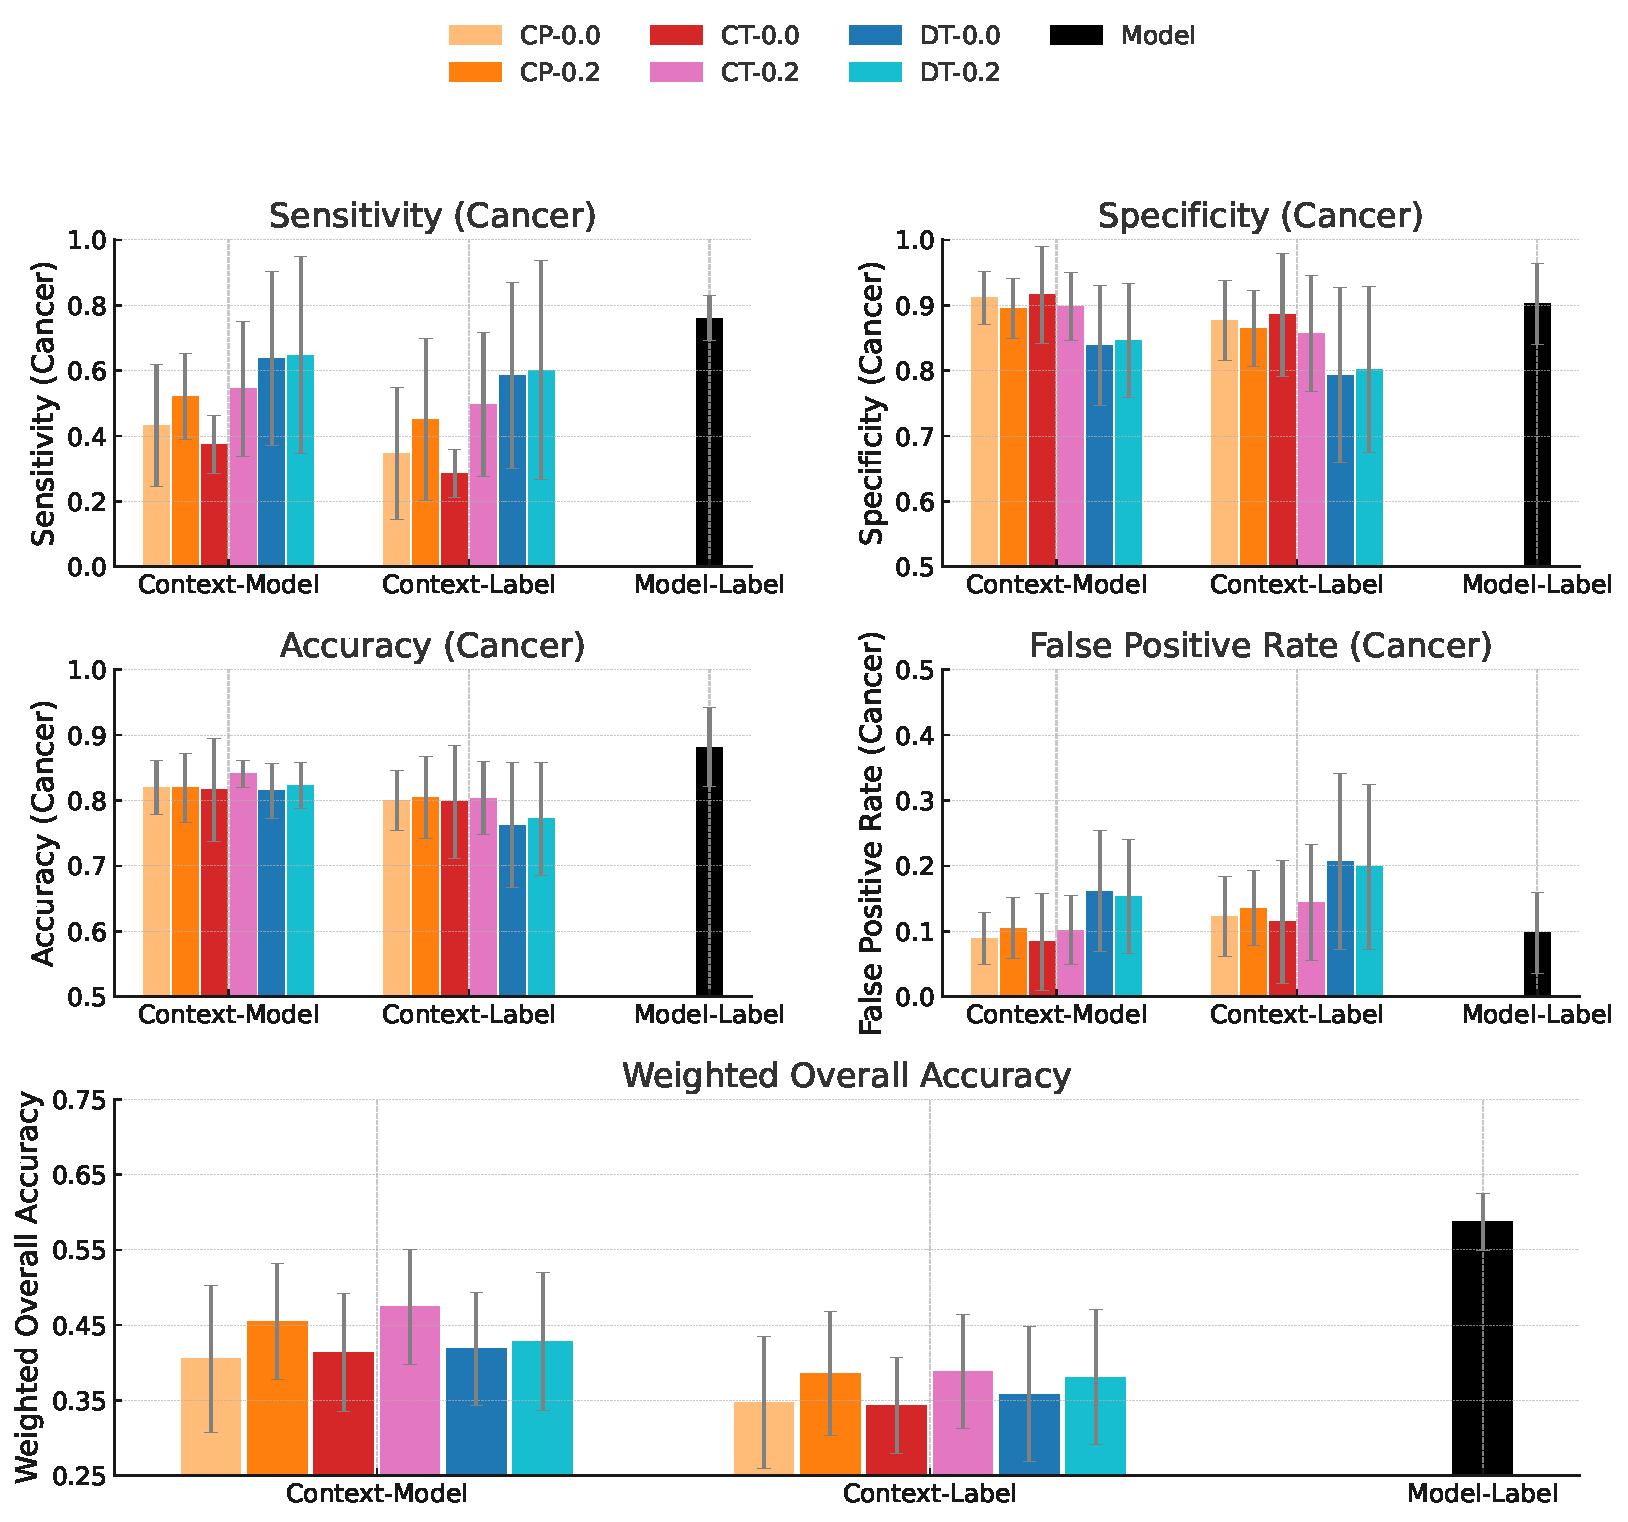
\includegraphics[width=1\textwidth]{Images/quad_class3_metrics_fig_updated4.pdf} 
    \caption{LCRIME four-class classification performance (mean $\pm$ std) across folds with $K=100$ clustering. The VAE model used is denoted using the convention outlined in Table \ref{tab:ssvae_arch}, followed by the decimalised value of the supervision level used.}
    \label{fig:quad_context}
\end{figure}

\begin{figure}
    \centering 
    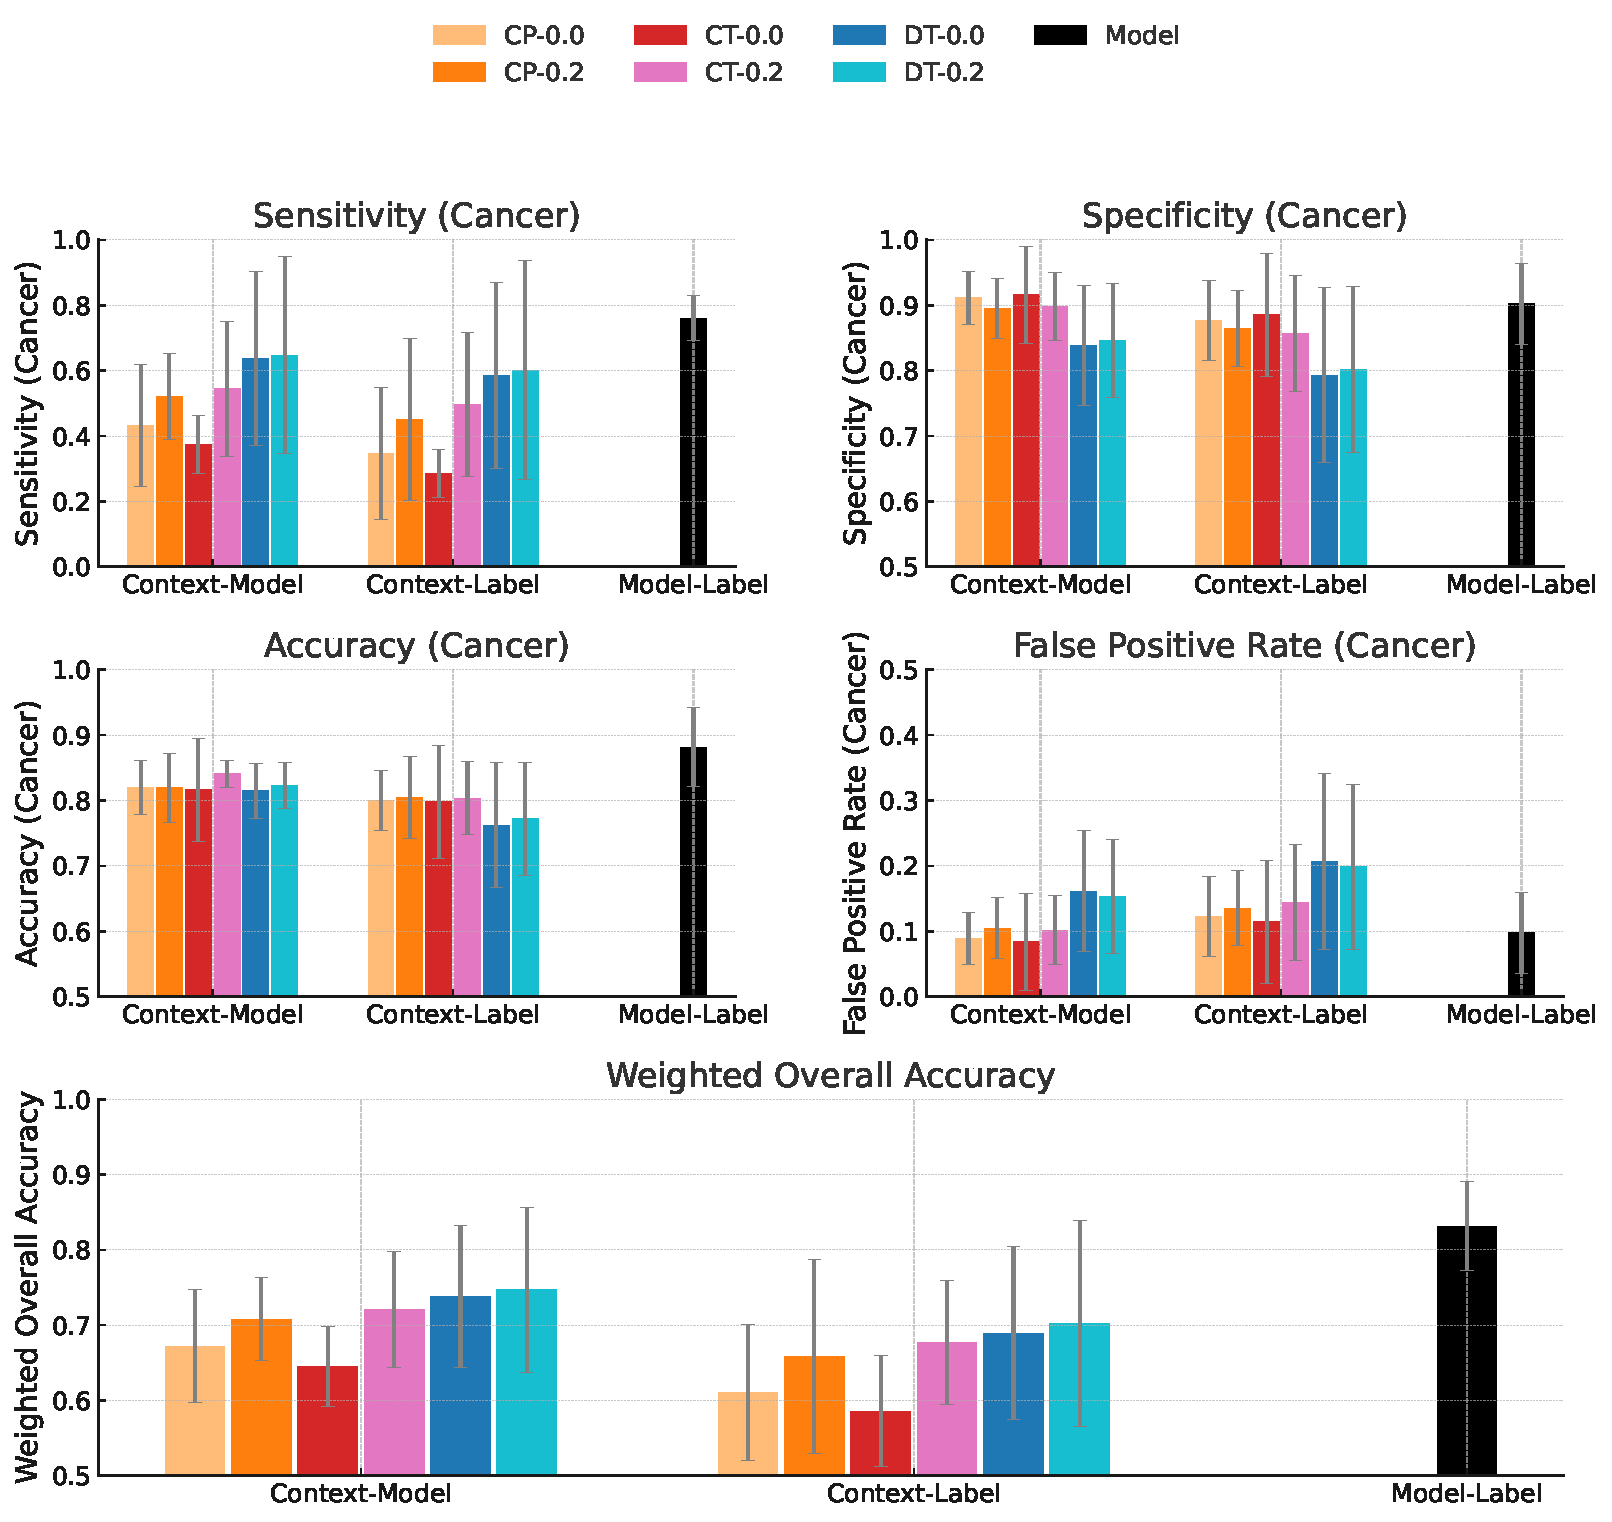
\includegraphics[width=1\textwidth]{Images/binary_metrics_fig_updated4.pdf} 
    \caption{LCRIME binary classification performance (mean $\pm$ std)
    across folds with $K=100$ clustering. The VAE model used is denoted using
    the convention outlined in Table \ref{tab:ssvae_arch}, followed by the
    decimalised value of the supervision level used.}
    \label{fig:bin_context}
\end{figure}

\subsection{Applicability in Physics}
The use of machine learning and deep learning methods is becoming increasingly common in physics. Similar approaches to the VAE method adopted here have been used to detect and reconstruct collisions in particle physics \cite{cheng_variational_2023,cerri_variational_2019,alves_variational_2024}, perform discovery and age-prediction tasks in astrophysical contexts \cite{andika_accelerating_2025, leung_variational_2023,gagliano_physics-informed_2023}, detect gravitational waves \cite{gabbard_bayesian_2022,bayley_rapid_2022,bayley_robust_2020,yamamoto_use_2020}, and perform cancer diagnosis and severity classification tasks in medical physics, as demonstrated and exemplified throughout this work. Increasing the interpretability of these methods, such as through the techniques illustrated in this work, is therefore important for translating new-found results, particularly within large datasets into real physical insights.

% \newpage